%%\documentclass[9pt,twocolumn]{jctc}   % two-column format
%\documentclass[9pt,twocolumn]{jpc}   % two-column format (WS: modify previous)
%%\documentclass[9pt,onecolumn]{jpc}  % one-column format
%%\renewcommand{\baselinestretch}{2.0} % double-spaced

%% We will be using PDF figures and generating PDF output.
%\pdfoutput=1
%\pdfcompresslevel=9
%\usepackage[pdftex]{graphicx}
%\DeclareGraphicsExtensions{.pdf}

%% The figures are in a figures/ subdirectory.
%\graphicspath{{figures/}}

%% Import useful packages.
%\usepackage{times}                             	   % nice fonts
%\usepackage{amsmath}                           % for 'case'
%\usepackage{amsthm}                             % for theorems and proofs
%\usepackage{mathrsfs}                            % script math font
%\usepackage{url}                                	   % allow use of URLs
%\usepackage{latexsym}                            % some math symbols, like \Box
%\usepackage{subfigure}                           % allow use of subfigures

%% Define some useful commands we will use repeatedly.
%\newcommand{\T}{\mathrm{T}}                                % T used in matrix transpose
%\newcommand{\tauarrow}{\stackrel{\tau}{\rightarrow}}       % the symbol tau over a right arrow
%\newcommand{\expect}[1]{\langle #1 \rangle}                % <.> for denoting expectations over realizations of an experiment or thermal averages
%\newcommand{\estimator}[1]{\hat{#1}}                       % estimator for some quantity from a finite dataset.
%\newcommand{\code}[1]{{\tt #1}}
%\newcommand{\bfm}[1]{{\bf #1}}              % proper boldface for math environment

%%% DOCUMENT %%%%%%%%%%%%%%%%%%%%%%%%%%%%%%%%%%%%%%%%%%%%%%%%%%%%%%%%%%%%%%%%%%%%
%\begin{document}

%%% TITLE %%%%%%%%%%%%%%%%%%%%%%%%%%%%%%%%%%%%%%%%%%%%%%%%%%%%%%%%%%%%%%%%%%%%
%\title{Automatic discovery of metastable states for the construction of Markov models of macromolecular conformational dynamics}

%\author{
%{\bf John D. Chodera$^{+\dag}$ and Ken A. Dill$^\ddag$} \\
%\emph{\normalsize $^\dag$Graduate Group in Biophysics and $^\ddag$Department of Pharmaceutical Chemistry, University of California, San Francisco, CA 94143} \vspace{0.1cm} \\
%{\bf Nina Singhal$^{+ \S}$ and Vijay S. Pande$^\P$} \\
%\emph{\normalsize $^{\S}$Department of Computer Science and $^\P$Department of Chemistry, Stanford University, Stanford, CA 94305} \vspace{0.1cm} \\ 
%{\bf William C. Swope\footnote{Author to whom correspondence should be addressed: William C. Swope {\tt <swope@us.ibm.com>}}$\ $} \\
%\emph{\normalsize IBM Almaden Research Center, 650 Harry Road, San Jose, CA 95120} \vspace{0.1cm} \\
%\emph{\normalsize $^+$ These authors contributed equally to this work.}
%}

%\maketitle
%\date{}

The material in this chapter will be submitted to the \emph{Journal of Chemical Physics} for publication as

\flushleft{\bf Automatic discovery of metastable states for the construction of Markov models of macromolecular conformational dynamics}

%\author{
%{\bf John D. Chodera$^{+\dag}$ and Ken A. Dill$^\ddag$} \\
%\emph{\normalsize $^\dag$Graduate Group in Biophysics and $^\ddag$Department of Pharmaceutical Chemistry, University of California, San Francisco, CA 94143} \vspace{0.1cm} \\
%{\bf Nina Singhal$^{+ \S}$ and Vijay S. Pande$^\P$} \\
%\emph{\normalsize $^{\S}$Department of Computer Science and $^\P$Department of Chemistry, Stanford University, Stanford, CA 94305} \vspace{0.1cm} \\ 
%{\bf William C. Swope\footnote{Author to whom correspondence should be addressed: William C. Swope {\tt <swope@us.ibm.com>}}$\ $} \\
%\emph{\normalsize IBM Almaden Research Center, 650 Harry Road, San Jose, CA 95120} \vspace{0.1cm} \\
%\emph{\normalsize $^+$ These authors contributed equally to this work.}
%}

\flushleft{
{\bf John D. Chodera$^{+1}$, Nina Singhal$^{+2}$, Vijay S. Pande$^3$, Ken A. Dill$^4$, and William C. Swope$^5$\footnote{Author to whom correspondence should be addressed: William C. Swope {\tt <swope@us.ibm.com>}}} \\
\emph{\normalsize $^1$Graduate Group in Biophysics and $^4$ Department of Pharmaceutical Chemistry, University of California, San Francisco, CA 94143} \\
\emph{\normalsize $^2$ Department of Computer Science and $^3$ Department of Chemistry, Stanford University, Stanford, CA 94305} \\ 
\emph{\normalsize $^5$ IBM Almaden Research Center, 650 Harry Road, San Jose, CA 95120} \\
\emph{\normalsize $^+$ These authors contributed equally to this work.}
}

%\begin{abstract}
\section*{Abstract}

To meet the challenge of modeling the conformational dynamics of biological macromolecules over long timescales, much recent effort has been devoted to constructing stochastic kinetic models, often in the form of discrete-state Markov models, from short molecular dynamics simulations.
To construct useful models that faithfully represent dynamics at the timescales of interest, it is necessary to decompose configuration space into a set of kinetically metastable states.
Previous attempts to define these states have relied upon either prior knowledge of the slow degrees of freedom or on the application of conformational clustering techniques which assume that conformationally distinct clusters are also kinetically distinct.
Here, we present a first version of an \emph{automatic} algorithm for the discovery of kinetically metastable states that is generally applicable to solvated macromolecules.
Given molecular dynamics trajectories initiated from a well-defined starting distribution, the algorithm discovers long-lived, kinetically metastable states through successive iterations of partitioning and aggregating conformation space into kinetically related regions.
We apply this method to three peptides in explicit solvent --- terminally blocked alanine, the engineered 12-residue $\beta$-hairpin trpzip2, and the 21-residue helical F$_s$ peptide --- to assess its ability to generate physically meaningful states and faithful kinetic models.

%\emph{Keywords: macromolecular conformational dynamics; protein folding; Markov chain; Markov state model; master equation model; molecular dynamics simulation; alanine dipeptide; trpzip2; Fs peptide}
%\end{abstract}

%% INCLUDE SECTIONS %%%%%%%%%%%%%%%%%%%%%%%%%%%%%%%%%%%%%%%%%%%%%%%%%%%%%%%%%%%%%%%%%%%%
%% INTRODUCTION %%%%%%%%%%%%%%%%%%%%%%%%%%%%%%%%%%%%%%%%%%%%%%%%%%%%%%%%%%%%%%%%
\section{Introduction}

% TODO: 
% -Footnote on inclusion of Jacobian correction
% - Do we cite the Aaron Dinner paper on the automatic discovery of reaction coordinates anywhere?
% - Add sentence here or in Theory: These barriers produce a memory effect, whereby trajectories that enter the state from one side of the barrier behave qualitatively differently from ones that enter from the other side, until an adequate amount of time has passed for many barrier crossing events within this state.  

Many biomolecular processes are fundamentally dynamic in nature.
Protein folding, for example, involves the ordering of a polypeptide chain into a particular topology over the course of microseconds to seconds, a process which can go awry and lead to misfolding or aggregation, causing disease \cite{dobson:nature:2003:misfolding}.
Enzymatic catalysis may involve transitions between multiple conformational substates, only some of which may allow substrate access or catalysis \cite{kern:science:2002,youngblood:jbc:2006a,boehr:2006a}.
Post-translational modification events, ligand binding, or catalytic events may alter the transition kinetics among multiple conformational states by modulating catalytic function, allowing work to be performed, or transducing a signal through allosteric change \cite{frauenfelder:pnas:2001,changeux:2005a,maki:jbc:2006a}.
A purely static description of these processes is insufficient for mechanistic understanding --- the dynamical nature of these events must be accounted for as well.

Unfortunately, these processes may involve molecular timescales of microseconds or longer, placing them well outside the range of typical detailed atomistic simulations employing explicit models of solvent.
Many of these systems are very large, limiting the length of trajectories that can be generated by molecular dynamics simulation.
However, due to the presence of many energetic barriers on the order of the thermal energy, the uncertainty in initial microscopic conditions, and the stochasticity introduced into the system by the surrounding solvent in contact with a heat bath, any suitable description of conformational dynamics must \emph{by necessity} be statistical in nature.
This has motivated the development of stochastic kinetic models of macromolecular dynamics which might conceivably be constructed from short dynamics simulations, yet provide a useful and accurate statistical description of dynamical evolution over long times. 

Several approaches have been used to construct of these models.
\emph{Transition interface sampling} (TIS) \cite{moroni:2004b}, \emph{milestoning} \cite{faradjian:2004a}, and methods based on commitment probability distributions \cite{rhee:2005a,berezhkovskii:2005a} attempt to describe dynamics along a one dimensional reaction coordinate, but these approaches are valid only if an appropriate reaction coordinate can be identified such that relaxation transverse to this coordinate is fast compared to diffusion along it.
Discrete-state, continuous-time master equation models, characterized by a matrix of phenomenological rate constants describing the rate of interconversion between states \cite{vankampen}, can be constructed by identifying local potential energy minima as states and estimating interstate transition rates by transition state theory \cite{czerminski:1990a,kunz:1995a,ball:1998b,levy:2001a,mortenson:2001a,mortenson:2002a,evans:2004a}.
Unfortunately, the number of minima, and hence the number of states, grows exponentially with system size, making the procedure prohibitively expensive for larger proteins or systems containing explicit solvent molecules.
Others have suggested that stochastic models of dynamics can be constructed by expansion of the appropriate dynamical operator in a basis set \cite{shalloway:1996a,ulitsky:1998a,shen:2003a}, but this approach appears to be limited by the great difficulty of choosing rapidly-convergent basis sets for large molecules, a process that is not fundamentally different from identifying the slow degrees of freedom.

Instead, much work has focused on the construction of discrete- or continuous-time Markov models to describe dynamics among a small number of states which may each contain many minima within large regions of configuration space \cite{grubmueller:1994a,degroot:2001a,swope:2004b,singhal:2004a,levy:2005a,sorin:2005b,sriraman:2005a,schultheis:2005a,singhal:2005a,elmer:2005b,park:2006a}.
In these models, it is hoped that a separation of timescales between fast \emph{intrastate} motion and slow \emph{interstate} motion allows the statistical dynamics to be modeled by stochastic transitions among the discrete set of metastable conformational states governed by first-order kinetics.
Such a separation of timescales would be a natural consequence of the widely held belief that the nature of the energy landscape of biomacromolecules is hierarchical \cite{ansari:1985a,bai:1989a,becker:1997a,levy:2001a,levy:2002a}.
If the system reaches local equilibrium \emph{within} the state before attempting to exit, the probability of transitioning to any other state will be independent of all but the current state.
This allows the process to be modeled with either a discrete-time Markov chain (e.g.\ Ref.\ \cite{singhal:2004a}) or a continuous-time master equation model with coarse-grained time (e.g.\ Ref.\ \cite{sriraman:2005a}).
In either model, processes occurring on timescales faster than a coarse-graining time, determined by the time to reach equilibrium within each state, cannot be resolved.

Markov models embody a concise description of the various kinetic pathways and their relative likelihood, facilitating comparison with experimental data and providing a powerful tool for mechanistic insight.
Once the model is constructed and the timescale for Markovian behavior determined, it can be used to compute the stochastic temporal evolution of either a single macromolecule or a population of noninteracting macromolecules, allowing direct comparison of simulated and experimental observables for both single-molecule or ensemble kinetics experiments.
In addition, useful properties difficult to access experimentally, such as state lifetimes \cite{swope:2004a}, relaxation from experimentally inaccessible prepared states \cite{chodera:mms:2006}, mean first-passage times \cite{singhal:2004a}, the existence of hidden intermediates \cite{ozkan:2002a}, and $P_\mathrm{fold}$ values or transmission coefficients \cite{lenz:2004a}, can easily be obtained.
This allows for both a thorough understanding of mechanism and the generation of new, experimentally testable hypotheses.

To build such a model, it is necessary to decompose configuration space into an appropriate set of metastable states.
If the low-dimensional manifold containing all the slow degrees of freedom is known a priori, then this can be partitioned into free energy basins to define the states, such as by examination of the potential of mean force \cite{swope:2004b,sriraman:2005a,sorin:2005b,elmer:2005b,chodera:mms:2006}.
In the absence of this knowledge, others have turned to conformational clustering techniques to identify conformationally distinct regions which may also be kinetically distinct \cite{karpen:1993a,degroot:2001a,singhal:2004a,levy:2005a}.

Instead, we adopt a strategy first suggested for the discovery of metastable states in biomolecular systems by researchers at the \emph{Konrad-Zuse-Zentrum f\"{u}r Informationstechnik} \cite{schuette:1999a}.
The principal idea is this: If configuration space could be decomposed into a large number of small cells, the probability of transitioning between these cells in a fixed evolution time could be measured.
This probability is a measure of \emph{kinetic connectivity} among the cells, which allows the identification of aggregates of these cells that approximate true metastable states \cite{schuette:2002b}.
Unfortunately, the choice of how to divide configuration space into cells is not straightforward.
Suppose one is to consider the analysis of some fixed amount of simulation data. 
If configuration space is decomposed very finely, the boundaries between metastable states can in principle be well-approximated, but the estimated cell-to-cell transition probabilities will become statistically unreliable.
On the other hand, if configuration space is decomposed too coarsely, the transition probabilities may be well-determined, but the boundaries between metastable states cannot be clearly resolved, potentially disrupting or destroying the Markovian behavior of interstate dynamics.
An optimal choice would ultimately require knowledge of the metastable regions in order to determine the best decomposition of space into cells.

In this work, we propose an iterative procedure to determine both the choice of cells and their aggregates to approximate the desired metastable states.
% JDC: Do we want to say how this differs from previously proposed methods, such as sequential dihedral PCCA, or self-organizing box maps?
We use a conformational clustering method to carve configuration space into an initial crude set of cells (\emph{splitting}), and a Monte Carlo simulated annealing procedure to collect metastable collections of cells into states (\emph{lumping}).
This cycle is repeated, with the splitting procedure now applied individually to each state to generate a new set of cells, and the lumping procedure applied to the entire set of cells to redefine states until further application of this procedure leaves the approximations to metastable states unchanged.
This procedure allows state boundaries to be iteratively refined, as regions that mistakenly have been included in one state can be split off and regrouped with the proper state.
Throughout this process, we require that the cells never become so small that estimation of the relevent transition matrix elements is statistically unreliable.
Our proposed method is efficient, of $\mathcal{O}(N)$ complexity in the number of stored configurations, and can be easily parallelized.

This paper is organized as follows:
In Section \ref{automatic:section:theory}, we give an overview of the Markov chain model and its construction, elaborate on desirable properties of an algorithm to partition configuration space into states, and outline the principles underlying the algorithm we present here.
In Section \ref{automatic:section:methods}, we provide a detailed description of the automatic state decomposition algorithm and its implementation.
In Section \ref{automatic:section:applications}, we apply this algorithm to three model peptide systems in explicit solvent to assess its performance: alanine dipeptide, the 12-residue engineered trpzip2 hairpin, and the 21-residue F$_s$ helix-forming peptide.
Finally, in Section \ref{automatic:section:discussion}, we discuss the advantages and shortcomings of our algorithm, with the hope that future state decomposition algorithms can address the remaining challenges.

%% THEORY %%%%%%%%%%%%%%%%%%%%%%%%%%%%%%%%%%%%%%%%%%%%%%%%
\section{Theory}
\label{automatic:section:theory}

% TODO:
% - Add a citation (e.g. van Kampen) for Chapman-Kolmogorov?
% - Add a section on validation using Chapman-Kolmogorov?

Some discussion of the stochastic model of kinetics considered here and the theory underlying the method is appropriate before describing the algorithmic implementation in detail.
First, in Section \ref{automatic:section:theory:markov-model-introduction}, we review Markov chain and master equation models of conformational dynamics.
Next, in Section \ref{automatic:section:theory:construction-from-simulation-data}, we describe their construction from equilibrium molecular dynamics trajectories given any state partitioning.
Section \ref{automatic:section:theory:requirements-for-markovian-behavior} enumerates a number of requirements for a useful state partitioning.
Finally, Section \ref{automatic:section:theory:validation} discusses possible methods for validating a given state decomposition.
The actual implementation of the algorithm used here is described in detail in Section \ref{automatic:section:methods}.

\subsection{Markov chain and master equation models of conformational dynamics.}
\label{automatic:section:theory:markov-model-introduction}

Consider the dynamics of a macromolecule immersed in solvent, where the solvent is at equilibrium at some particular temperature of interest.
We presume that all of configuration space has already been decomposed into a set of nonoverlapping regions, or \emph{states}, which together form a complete decomposition of configuration space.
The method by which these states are identified is described in subsequent sections.

If we observe the evolution of this system at times $t = 0, \tau, 2 \tau, \ldots$, where $\tau$ denotes the observation interval, we can represent this sequence of observations in terms of the state the system visits at each of these discrete times.
The sequence of states produced is a realization of a \emph{discrete-time stochastic process}.
For this process to be described by a Markov chain, it must satisfy the \emph{Markov property}, whereby the probability of observing the system in any state in the sequence is independent of all but the previous state.
For a stationary process on a finite set of $L$ states, this process can be completely characterized by an $L \times L$ \emph{transition matrix}\footnote{We adopt the notation for a \emph{column-stochastic} transition matrix, in which the columns sum to unity.  This differs from the notation in some previously-cited references, which use a \emph{row stochastic} transition matrix, equal to the transpose of the column stochastic matrix used here.} $\bfm{T}(\tau)$ dependent only on the observation interval, or \emph{lag time}, $\tau$.
The element $T_{ji}(\tau)$ denotes the probability of observing the system in state $j$ at time $t$ given that it was previously in state $i$ at time $t-\tau$.
If this process satisfies detailed balance (which we will assume to be the case for physical systems of the sort we consider here \cite{vankampen}) we additionally have the requirement
\begin{eqnarray}
T_{ji} p_{\mathrm{eq},i} = T_{ij} p_{\mathrm{eq},j}
\end{eqnarray}
where $p_{\mathrm{eq},i}$ denotes the equilibrium probability of state $i$.

The vector of probabilities of occupying any of the $L$ states at time $t$ (here also referred to as the vector of state populations, such as in an experiment involving a population of noninteracting macromolecules) can be written as $\bfm{p}(t)$.
If the initial probability vector is given by $\bfm{p}(0)$, we can write the probability vector at some later time $t=n\tau$ as
\begin{eqnarray}
\bfm{p}(n \tau) \: = \: \bfm{T}(n \tau) \bfm{p}(0) \: = \: [\bfm{T}(\tau)]^n \bfm{p}(0) . \label{automatic:equation:chapman-kolmogorov}
\end{eqnarray}
This is a form of the \emph{Chapman-Kolmogorov equation}.

Alternatively, the process can be characterized in {\em continuous} time by a matrix of phenomenological rate constants $\bfm{K}$, where the element $K_{ji}$, $j \ne i$ denotes the nonnegative phenomenological rate from state $i$ to state $j$.
The diagonal elements are determined by $K_{ii} = - \sum_{j \ne i} K_{ji}$ to ensure the columns sum to zero so as to conserve probability mass.
Time evolution is then governed by the equation
\begin{eqnarray}
\dot{\bfm{p}}(t) &=& \bfm{K} \bfm{p}(t) \label{automatic:equation:master-equation}
\end{eqnarray}
where the dot represents differentiation with respect to time.
This evolution equation has formal solution
\begin{eqnarray}
\bfm{p}(t) &=& e^{\bfm{K} t} \bfm{p}(0) \label{automatic:equation:master-equation-evolution} ,
\end{eqnarray}
where the exponential denotes the formal matrix exponential.
Eq.\ \ref{automatic:equation:master-equation} is often referred to as a \emph{master equation} \cite{vankampen,oppenheim:1977a} describing evolution among a discrete set of states in continuous time.
It is important to note that, despite the fact that $\bfm{p}(t)$ is formally defined for all times $t$, we do not expect Eq.\ \ref{automatic:equation:master-equation-evolution} to hold for \emph{all} times $t$ for physical systems of the sort we consider here.
In particular, for states of finite extent in configuration space, there exists a corresponding limit for the time resolution for which dynamics will appear Markovian; processes that occur on timescales shorter than this will be be incorrectly described by the master equation.
We will return to this topic in detail in subsequent sections.

There is an obvious relationship between the transition matrix $\bfm{T}(\tau)$ and the rate matrix $\bfm{K}$ evident from comparison of Eqs. \ref{automatic:equation:chapman-kolmogorov} and \ref{automatic:equation:master-equation-evolution}:
\begin{eqnarray}
\bfm{T}(\tau) &=& e^{\bfm{K} \tau} . \label{automatic:equation:relation-between-transition-and-rate-matrices}
\end{eqnarray}
If the process can be described by a continuous-time Markov process at all times, then this process can be equivalently described at discrete time intervals by the corresponding transition matrix.
The converse may not always be true due to sampling errors in $\bfm{T}(\tau)$, though methods exist to recover rate matrices $\bfm{K}$ consistent with the observed data and the requirements of detailed balance and nonnegativity rates \cite{grubmueller:1994a,sriraman:2005a}.

The transition and rate matrices have eigenvalues $\mu_k(\tau)$ and $\lambda_k$, respectively, and share corresponding right eigenvectors $\bfm{u}_k$.
The detailed balance requirement additionally ensures that all eigenvalues are real, and we here presume them to be sorted in descending order.
%The transition and rate matrices have related eigenvalue decompositions
%\begin{eqnarray}
%\bfm{K} = \bfm{U} \, \bfm{\Lambda} \, \bfm{U}^{-1} \: &;& \: \bfm{T(\tau)} = \bfm{U} \, \bfm{M}(\tau) \, \bfm{U}^{-1}
%\end{eqnarray}
%where the diagonal matrix $\bfm{\Lambda}$ contains the eigenvalues $\lambda_k$ of $\bfm{K}$, the diagonal matrix $\bfm{M}(\tau)$ contains the eigenvalues $\mu_k(\tau)$ of $\bfm{T(\tau)}$, and $\bfm{U}$ contains the eigenvectors as column vectors.
$\mu_k(\tau)$ and $\lambda_k$ are related by
\begin{eqnarray}
\mu_k(\tau) &=& e^{\lambda_k \tau} . \label{automatic:equation:implied-timescales-relation}
\end{eqnarray}
%For indecomposable Markov chains, for which the transition matrix is ergodic, there will be exactly one eigenvalue $\mu_1$ of unity (or equivalently $\lambda_1 = 0$), and its corresponding right eigenvector $\bfm{u}_1$ will contain the invariant equilibrium distribution (when properly normalized such that $\bfm{1}^\T \bfm{u}_1 = 1$).
%As the dynamical evolution of the system in continuous time can be expanded in terms of the eigenvectors as
%\begin{eqnarray}
%\bfm{p}(t) &=& \sum_{k=1}^M (\bfm{u}_k, \bfm{p}(0)) \, e^{\lambda_k t} \, \bfm{u}_k
%\end{eqnarray}
%where $(\bfm{a},\bfm{b}) = \sum_i p_{\mathrm{eq},i}^{-1} \, a_i \, b_i$ denotes the inner product \cite{vankampen}
The eigenvalues each imply a timescale corresponding to an inverse aggregate rate
\begin{eqnarray}
\tau_k = - \lambda_k^{-1} = - \tau [ \ln \mu_k(\tau) ]^{-1} \label{automatic:equation:implied-timescales}
\end{eqnarray}
and the associated eigenvector gives information about the aggregate conformational transitions that are associated with this timescale \cite{schuette-thesis,schuette:1999a,huisinga-thesis,schuette:2002a}.
In particular, the components of $\bfm{u}_k$ sum to zero for each $k \ge 2$, and the aggregate dynamical mode can be identified with transitions from microstates with positive eigenvector components interconverting with the set of microstates with negative components, and vice-versa, with the degree of participation in the mode governed by the magnitude of the eigenvector component.
This fact can be useful in deducing the conformational transitions among aggregated regions of configuration space that govern relaxation to equilibrium, which is achieved once all processes have exponentially damped out.

For the remainder of this manuscript, we will refer exclusively to the discrete-time Markov chain model picture without loss of generality (Eq.\ \ref{automatic:equation:chapman-kolmogorov}), except for use of the timescales implied by the transition matrix, as described above.
% JDC: Add reference to Mori-Zwanzig paper, if finished in time, discussing addition properties that K and T must have for physical systems, as a consequence of the projection operator formalism.

\subsection{Construction from simulation data given a state partitioning.}
\label{automatic:section:theory:construction-from-simulation-data}

Once a statistical-mechanical ensemble describing equilibrium and a microscopic model describing dynamical evolution in phase space have been selected, the transition matrix $\bfm{T}(\tau)$ can be estimated from molecular dynamics simulations.
For a system in which dynamical evolution is Newtonian and, at equilibrium, configurations are distributed according to a canonical distribution at a given temperature, Swope \emph{et al.}\cite{swope:2004a} show that the transition probability $T_{ji}(\tau)$ can be written as the following ratio of canonical ensemble averages:
\begin{eqnarray}
T_{ji}(\tau) 
%&\equiv& \int d\bfm{z}(0) \, p_i(\bfm{z}(0)) \, \chi_j(\bfm{z}(\tau)) \label{automatic:equation:transition-element-conditional-probability} \\
&=& \frac{\int d\bfm{z}(0) \, e^{-\beta H(\bfm{z}(0))} \, \chi_j(\bfm{z}(\tau)) \, \chi_i(\bfm{z}(0))}{\int d\bfm{z}(0) \, e^{-\beta H(\bfm{z}(0))} \, \chi_i(\bfm{z}(0))} \label{automatic:equation:transition-element-phase-space-integrals} \\
&=& \frac{\expect{\chi_j(\tau) \chi_i(0)}}{\expect{\chi_i}} \label{automatic:equation:transition-element-correlation-functions}
\end{eqnarray}
where $\bfm{z(t)}$ denotes a point in phase space visited by a trajectory at time $t$, 
$\chi_i(\bfm{z})$ denotes the indicator function for state $i$ (which assumes a value of unity if $\bfm{z}$ is in state $i$, and zero otherwise),
%$p_i(\bfm{z})$ the equilibrium distribution confined within state $i$, 
$\beta \equiv (k_B T)^{-1}$ the inverse temperature, $H(\bfm{z})$ the Hamiltonian, and $\left< A \right>$ the canonical ensemble expectation of a phase function $A(\bfm{z})$ at inverse temperature $\beta$.

Given a set of simulations initiated from an equilibrium distribution, the expectations in Eq.\ \ref{automatic:equation:transition-element-correlation-functions} can be computed independently by standard analysis methods \cite{allen:1991a}.
Estimation of the correlation function in the numerator can make use of both the stationarity of an equilibrium distribution (by considering overlapping intervals of time $\tau$), and the microscopic reversibility (by considering also time-reversed versions of the simulations) 
of Newtonian trajectories.
Alternatively, if an equilibrium distribution within each state can be prepared, one can also directly estimate a column of transition matrix elements by computing the fraction of trajectories initially at equilibrium within state $i$ that terminate in state $j$ a time $\tau$ later.
More elaborate methods based on equilibrium ensembles prepared within special \emph{selection cells} that are not coincident with the states \cite{swope:2004a,swope:2004b} or \emph{partition of unity} restraints \cite{weber-thesis:2006a} can also be used to compute transition matrix elements efficiently.

\subsection{Requirements for a useful Markov model.}
\label{automatic:section:theory:requirements-for-markovian-behavior}
% JDC: In light of Bill's change of the focus of this section, we should change its title to something like "Further requirements for chemical insight.."?

For any given state partitioning, the dynamics of the system will be Markovian on some time scale.
For example, if the lag time $\tau$ is so long as to approach the time for the system to relax to an equilibrium distribution from any arbitrary nonequilibrium starting distribution, a single application of the transition matrix $\bfm{T}(\tau)$ carries any arbitrary initial probability distribution directly to the invariant equilibrium distribution.
However, if this $\tau$ exceeds the timescale of the process of interest, our model is not useful\footnote{Equilibrium probabilities can still be extracted from the stationary eigenvector (the eigenvector of corresponding to an eigenvalue of unity) of such a transition matrix, which may have some utility if one had constructed the transition matrix from trajectories not initiated from distributions at equilibrium globally.} for describing it, and therefore it is advantageous to attempt to find a state decomposition that is Markovian on a shorter timescale in order to extract useful dynamical information about this process. 

For a given state $i$, we will define its internal equilibration time, $\tau_{\mathrm{int},i}$, as the characteristic time one must wait before the system, initially in a configuration within state $i$, generates a new \emph{uncorrelated} configuration within the state by dynamical evolution.
This internal equilibration time, or \emph{memory time}, closely related to the molecular relaxation timescale $\tau_\mathrm{mol}$ in Chandler's reactive flux formulation of transition state theory \cite{chandler:1978a}, depends, of course, on the choice of state decomposition.
We can denote the longest of these times over all states by $\tau_\mathrm{int}$.
This is not to be confused with the time it takes an arbitrary nonequilibrium distribution to relax to global equilibrium, but rather, the minimum lag time for which dynamics will appear to be Markovian using this particular state decomposition.  If the lag time is longer than $\tau_\mathrm{int}$, we will expect the system to have lost memory of its previous location within {\em any} state it may have been in, either remaining within that state or transitioning to a new one, and for dynamics on this set of states to be independent of history.
On the other hand, for lag times shorter than $\tau_\mathrm{int}$, we cannot guarantee that transition probabilities are independent of history everywhere.
This suggests a way in which the utility of various decompositions can be measured.
For a fixed number of states, the most useful model will partition configuration space to yield the shortest $\tau_\mathrm{int}$, as this model can be used to study the widest range of dynamical processes.
% JDC: Add something about how a lower bound on tau_int could be estimated from restrictions of Markov chains.  Cite Schuette papers on this.

%In order for the dynamical evolution of a macromolecule to resemble a Markov process, 
%we expect a number of conditions to be met.
%Mathematically, the only true requirement is history independence, 
%but a model that satisfies only this criteria may not be useful for the study of dynamical processes; 
%pathological cases can be constructed in which history dependence is strictly satisfied but the 
%resulting states have no physical meaning.
% JDC: I have Nina's example in the following sentence, but it may be too confusing to include.
% For example, if each state consisted of a large number of randomly assigned regions of phase space, 
%the resulting model will likely be Markovian at short times, but a single application of the 
%transition matrix will carry the system to equilibrium and the states would be meaningless.
In addition to producing transition probabilities that are history independent at a relevant lag time, we impose additional conditions on our states to ensure the resulting model also provides physical and chemical insight.
Because we are primarily interested in macromolecular dynamical motion such as protein folding, we first require that states be consistent with a chemical intuition for a macromolecular {\em conformational} substate and, therefore, exist as constructs exclusively in the configuration space of the macromolecule.
In solvated systems, we expect relaxation and decorrelation of momenta to be much faster than any of the dynamical behaviors of interest, and so we ignore momenta in defining our states.  
Furthermore, we presume reorganization of the solvent is faster than processes of interest, and therefore ignore coordinates associated with the surrounding solvent\footnote{We recognize that solvent coordinates may be critical in some phenomena, but dealing with solvent degrees of freedom would also require accounting for the indistinguishability of solvent molecules upon their exchange.  We leave this to further iterations of the algorithm.}.

%The fundamental assumption leading macromolecular dynamics to resemble a discrete-state Markov model 
%is the existence of a \emph{separation of timescales}.
Also, we seek conformational states that exhibit a {\em separation of timescales}.
If states can be constructed where the timescale for equilibration \emph{within} each state is much shorter than the timescale for transitions \emph{among} the states, we would expect interstate dynamics to be well-modeled by a Markov chain after sufficiently long observation intervals.
Consider, for example, the isomerization of butane, which has three main metastable conformational states (\emph{gauche-plus}, \emph{gauche-minus}, and \emph{trans}).
At sufficiently low temperature, dynamics is dominated by long dwell times \emph{within} each of these three states, punctuated by infrequent transitions between them.  
The slow interstate transition process is well-described by first order reaction kinetics for observation intervals longer than the fast molecular relaxation time for intrastate dynamics due to the presence of a separation of timescales \cite{chandler:1978a}.

In order for the states to be defined such that equilibration within a state is rapid, we further require that the region of configuration space defining each state be \emph{compact} and \emph{connected}.
% JDC: Nina had a concern regarding states that consist of unconnected regions related by symmetry, 
%but I can't quite recall the argument.  We may need to think about this some more.
A state composed of two or more unconnected regions of phase space defies the assumption that equilibration within the state is much faster than the characteristic time to leave it.
%While it may still be possible to construct cases where states are not contiguous yet the 
%resulting model is Markovian, we feel that this contiguity requirement is essential for the 
%states to be endowed with chemical or physical meaning.

%Another consequence of requiring rapid intrastate equilibration is that the probability of 
%transitioning to another state must be independent of the initial microscopic configuration within the state.
%In the Markov chain literature, this condition is called \emph{lumpability} \cite{kemeney:1960a}.
%While this could be directly tested by initiating many trajectories with random initial velocities 
%from each of a number of points within the state, this approach is impractical.
% JDC: Is more needed here?  Does this paragraph serve a specific purpose?

% JDC: We might add something about 'best' decomposition giving the slowest rates, by analogy with 
%variational TST.  To do this, we first need to introduce the concept of implied timescales, which 
%we do below in the Validation section.  This would require a bit of rewriting to introduce earlier.

% JDC: Metastable states appear relatively invariant with lag time tau (cite ZIB?) though use of 
%long enough tau will actually wipe out weakly metastable states.  Suggests we want to use a tau 
%less than or equal to the timescale of the processes of interest.  This tau does not have to 
%correspond to tau_eq, since this will be estimated in a separate step after the partitioning has 
%been selected (see Validation).

%To summarize, we have the following requirements:
%[WS: including this list seems redundant.]
%\begin{description}
%  \item [Compactness and connectivity.]  States consist of connected, compact regions in the configuration 
%space of the macromolecule.
%  \item [Separation of timescales.]  For each state, the internal equilibration time $\tau_\mathrm{eq}$ 
%is much shorter than the characteristic state lifetime $\tau_\mathrm{lifetime}$.  Maximizing the 
%metastability (Eq. \ref{automatic:equation:metastability}) may provide an inexpensive way to attempt to 
%achieve a separation of timescales.
%  \item [Utility.]  The internal equilibration time for the entire system, $\tau_\mathrm{eq}$, must be 
%shorter than the timescale of the fastest phenomenon of interest, $\tau^*$.
%\end{description}

\subsection{Validation of Markov models.}
\label{automatic:section:theory:validation}

Once a decomposition of configuration space is chosen, we are faced with the task of determining the observation time interval $\tau$ at which dynamics in this state space appears Markovian.
Unfortunately, we cannot directly compute the internal macrostate equilibration times, though examination of the eigenvalues of the transition matrix restricted to a state may give a lower bound on this time in the absence of statistical uncertainty \cite{meerbach:2004a}.
The most rigorous test for Markovian behavior would be a direct test for history independence.
The simplest test of this type is to compute second order transition probabilities and compare them to the appropriate products of the first order transition probabilities to see if their disagreement is statistically significant, though this would miss possible yet unlikely higher order history dependencies.
While it is possible to estimate these from the simulation data, this requires the estimation of three-time correlation functions, which often possess statistical uncertainties so large as to render them useless for this kind of test \cite{chodera:jpcb:2006}.

Raising the transition matrix to a power $n$ (hence summing over the intermediate states) and comparing with the observed transition probabilities for a lag time of $n\tau$, such that one is effectively determining whether the Chapman-Kolmogorov equation (Eq.\ \ref{automatic:equation:chapman-kolmogorov}) is satisfied, helps to reduce the uncertainty so that the test becomes practical.
This is equivalent to propagating the population in time out of a probability distribution confined to each state $i$ initially, and comparing the model evolution with the observed transition probabilities over times much longer than $\tau_{\mathrm{int}}$.
This serves as a check to ensure that the model is at least consistent with the dataset from which it was constructed, to within the statistical uncertainty of the transition matrices obtained from the dataset.
This method was employed, for example, in Refs.\ \cite{swope:2004a,chodera:mms:2006}.

Another approach, from Park, \emph{et al.}, \cite{park:2006a} uses concepts from information theory to compute the \emph{conditional mutual information} conveyed by the second-to-last state, which quantifies the discrepancy between observed second-order transition probabilities and the estimate modeled from first-order transition probabilities.
The result of this analysis is a scalar that quantifies the degree of history dependence.  
For a pure first-order Markov process, the mutual information will be zero, as no additional information is gained by including additional history.
While this method also requires computing three-time correlation functions, which may individually have substantial uncertainties, the weighted combination of these into a single value reduces the uncertainty in the resulting metric.
Unfortunately, there is no rigorous criteria for how small this measure must be in order for the model to be considered acceptably Markovian.

Swope, \emph{et al.}, \cite{swope:2004a} suggested a number of additional tests for signatures of Markov behavior, the most sensitive of which appears to be examining the behavior of the \emph{implied timescales} of the transition matrix $\bfm{T}(\tau)$, which can be computed from the eigenvalues of the transition matrix by Eq.\ \ref{automatic:equation:implied-timescales}, as a function of increasing lag time $\tau$ \cite{chodera:jpcb:2006}.
At sufficiently large $\tau$, the implied timescales will be independent of $\tau$, implying that exponentiation of the transition matrix is nearly identical to constructing the transition matrix using longer observation time intervals (Eq.\ \ref{automatic:equation:chapman-kolmogorov}).
% JDC: One primary criticism of Marcus Weber and the ZIB folks is that this is formally incorrect for our dynamical model, since repeated application of T(\tau) introduces a velocity randomization every \tau, whereas T(n\tau) only has a velocity randomization at time zero.  We note that it will only appear to be the case under particular conditions that permit such a model to describe kinetics.
The shortest observation time interval for which this holds can be correlated with the internal equilibration time $\tau_\mathrm{int}$, and descriptions of the behavior of the system using that state decomposition should be Markovian for all lag times $\tau \ge \tau_\mathrm{int}$.
This is also a test of whether the Chapman-Kolmogorov equation holds, but as it computes only $L$ numbers and orders them by timescale, it allows emphasis to be placed on the longest timescales in the system.

Unfortunately, this method has some drawbacks.  
First, small uncertainties in the eigenvalues of the transition matrix can induce very large uncertainties in the implied timescales.  
With increasing lag time $\tau$, the number of statistically independent observed transitions, from which $\bfm{T}(\tau)$ is estimated, diminishes, and the statistical uncertainty in the implied timescales $\tau_k$ will grow.
Second, while stability of the implied timescales with respect to lag time is a \emph{necessary} consequence of history independence, it is not itself \emph{sufficient} to guarantee history independence, though we may be unlikely to encounter physical systems for which this is problematic.
% NS: Another possible drawback is that since we calculate the implied time scales for increasing lag times, the end effects (especially when we have few trajectories that visit given states) may affect the results.  I think comparing only consecutive lag times are less sensitive to this, but we never really proved that this was why our timescales for low population states occasionally kept increasing
% JDC: Good point.  We need to get a handle on these end effects, if they are real.  Perhaps we should only be allowed to compute the timescales up to a lag time of half the longest trajectory length?  What if we have trajectories of a distribution of lengths?
However, tests on simple models indicate that the information theoretic metric suggests the emergence of Markovian behavior on similar lag times to this method, suggesting some degree of fundamental equivalence \cite{park:2006a}.

In this work, the analysis of implied timescales as a function of lag time will be our primary test for the emergence of Markovianness.

%From tests on simple models, comparison of analyses based on implied timescales and the information theoretic based metric appears to indicate the emergence of Markovian behavior at approximately the same lag time \cite{park:2006a}, and, so, the primary validation tests used in this work will be based on the analysis of implied timescales.

%Instead of testing for one- or two-time history independence of the transition probabilities, in some cases, it is also possible to test the statistical time evolution out of each state over longer times.
%An ensemble of starting conformations representative of some nonequilibrium condition could be prepared, and numerous simulations conducted to examine the statistical time evolution over long times.  
%The temporal behavior of the state populations as this ensemble relaxes to equilibrium should be consistent with that predicted by the model through repeated application of the transition matrix to the initial state probabilities.  
%%This would be of interest in the study of protein (un)folding experiments, such as laser temperature-jump experiments, in which a short laser pulse rapidly heats the solvent, taking the population of macromolecules out of equilibrium with respect to the higher temperature.
%%Although the models described in this work are constructed from equilibrium data characteristic of a particular temperature, we would expect to capture the dynamics of systems thermally perturbed in this way.
%% JDC: What about systems perturbed in other (non-thermal) ways?  My point was to stress that the model is only useful for particular perturbations away from equilibrium, and not ANY arbitrary perturbation from equilibrium.  I think we need to make this point.
%In this work, among other tests, we monitor the evolution of various ensembles of trajectories, selected from equilibrium but all started from a single state.
%We compare their evolution with a model constructed from trajectories at equilibrium.
%% JDC: What do we do here?

%% METHODS %%%%%%%%%%%%%%%%%%%%%%%%%%%%%%%%%%%%%%%%%%%%%%%%
\section{The automatic state decomposition algorithm}
\label{automatic:section:methods}

% TODO:
%  - caption for algorithm flowchart
%  - citation for why conformational averaging is bad

Based on the theory above, we provide a list of practical considerations for an automatic state decomposition algorithm and then present an algorithm that meets the criteria proposed below.
The algorithm operates on an ensemble of molecular dynamics trajectories where conformations (the Cartesian coordinates of all atoms of the macromolecule) have been stored at regular intervals.
In this work, we apply the method to a set of \emph{equilibrium} trajectories at the temperature of interest, but the algorithm can in principle be applied to trajectories generated from \emph{biased} initial conditions, provided the unbiased transition probabilities between regions of configuration space can be computed.
We stress that the algorithm presented here is simply a first attempt at a truly general and automatic algorithm for use with biomacromolecules. 

\subsection{Practical considerations for an automatic state decomposition algorithm.}
\label{automatic:section:methods:desiderata}

There are several desirable properties that a state decomposition should possess to be both useful and practical:
\begin{enumerate}
  \item It is not uncommon for simulations conducted on supercomputers such as Blue Gene \cite{fitch:2003a,germain:2005a}, distributed computing platforms such as Folding@Home \cite{pande:2000a,pande:2003a}, or even computer clusters to generate datasets that may contain $10^5$ to $10^7$ configurations in up to $10^4$ trajectories, therefore prohibiting the use of any algorithm with a time complexity greater than $\mathcal{O}(N \log N)$ in the number of configurations.
  \item Molecules may have symmetries under permutation of atoms, such as aromatic rings, the protons on methyl groups, and the oxygens of carboxylate groups that should be accounted for in some way.
  \item The state decomposition algorithm should produce a decomposition for which dynamics appears to be Markovian at the shortest possible lag time $\tau$, so as to produce the most useful model.
  \item The resulting model should not generate so many states so that the elements of the transition matrix will be statistically unreliable.
\end{enumerate}

\subsection{Sketch of the method.}
\label{automatic:section:methods:sketch}

\begin{figure}[tb]
  \begin{center}
    \resizebox{3.375in}{!}{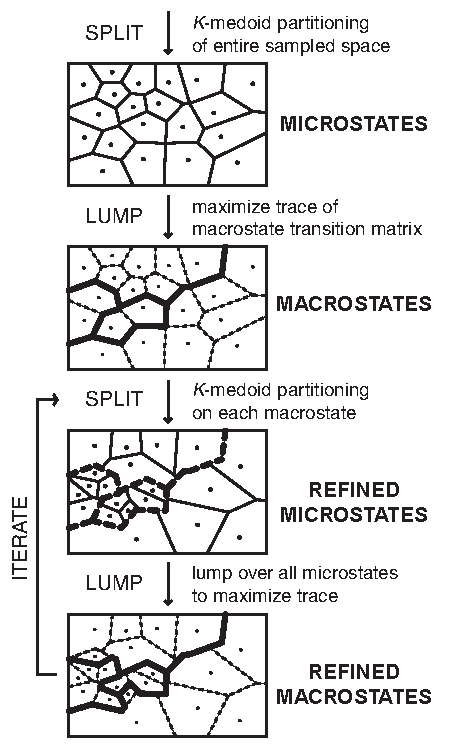
\includegraphics{chapters/automatic-state-decomposition/figures/flowchartsmall.pdf}}    
  \end{center}
  \caption{{\bf Flowchart of the automatic state decomposition algorithm.}}
  \label{automatic:figure:methods-flowchart}
\end{figure}

A state decomposition algorithm intended to produce the most \emph{useful} models, as discussed in Section \ref{automatic:section:theory:requirements-for-markovian-behavior} above, would generate models that minimize the internal equilibration time $\tau_\mathrm{int}$, the minimum time for which the model behaves in a Markovian fashion.
Unfortunately, $\tau_\mathrm{int}$ is difficult to determine directly, so we are instead forced to identify some surrogate quantity whose maximization will hopefully lead to improved separation between fast intrastate and slow interstate timescales.
Following the approach of Ref.\ \cite{huisinga:2005a}, we define a measure of the \emph{metastability} $Q$ of a partitioning into $L$ \emph{macrostates} as the sum of the self-transition probabilities for a given lag time $\tau$:
\begin{eqnarray}
Q &\equiv& \sum_{i=1}^L T_{ii}(\tau) \label{automatic:equation:metastability}
\end{eqnarray}
For $\tau = 0$, $Q = L$, and decays to unity as $\tau$ grows large enough for the self-transition probabilities $T_{ii}$ to reach the equilibrium probabilities of each macrostate.
Poor partitionings into weakly metastable states will result in a small $Q$, as trajectories started in some states will rapidly exit; conversely, good partitionings into strongly metastable states will result in a large $Q$, as trajectories will remain in each macrostate for long times.
In the absence of statistical uncertainty, $Q$ is bounded from above by the sum of the $L$ largest eigenvalues of the true dynamical propagator for the system \cite{huisinga:2005a}.

The goal of our algorithm is to identify a partitioning into $L$ contiguous macrostates that maximizes the metastability $Q$.
While in principle, the boundaries between these macrostates can be varied directly to optimize $Q$, in analogy to variational transition state theory \cite{truhlar:1996a}, a complicated parameterization may be necessary to describe the potentially highly convoluted hypersurfaces separating the states, and $Q$ may have multiple maxima in these parameters.
Instead, we choose an approach based on \emph{splitting} the conformation space into a large number of small contiguous \emph{microstates} and then \emph{lumping} these microstates into macrostates in such a way that maximizes the metastability.
% During this process, we choose some lag time $\tau$ that is less than or equal to the fastest timescale of interest.

This approach is very similar to the approach of Sch\"{u}tte and coworkers described in Ref.\ \cite{schuette:1999a}, but with a substantial difference.
In their work, each degree of freedom of the molecule (such as a torsion angle) is subdivided independently to produce a multidimensional grid.
As the number of states is exponential in the number of degrees of freedom, this approach quickly becomes intractable for macromolecules that possess large numbers of degrees of freedom, even if the sparsity of the transition matrix is taken into account.
Instead, we choose to let the data define the low-dimensional manifold of configuration space accessible to the macromolecule, and we can apply any clustering algorithm that is no worse than $\mathcal{O}(N \log N)$ in the number of configurations to decompose the sampled conformation space into a set of $K$ contiguous microstates.
This step corresponds to the first \emph{split} step in Figure \ref{automatic:figure:methods-flowchart}.

Once the conformation space is divided into $K$ microstates, we \emph{lump} the microstates together to produce $L < K$ macrostates with high metastability, $Q$.
This corresponds to the first \emph{lump} step in Figure \ref{automatic:figure:methods-flowchart}.  
% As described in Section \ref{automatic:section:theory:construction-from-simulation-data}, we can calculate a transition probability matrix for any decomposition of configuration space.
% The \emph{lump} step illustrated in Figure \ref{automatic:figure:methods-flowchart} combines the $K$ microstates into $L$ macrostates, calculates the new transition matrix between the macrostates, and chooses a lumping with high metastability.
The difficulty here is that the uncertainty in the metastability of a partitioning can be large if any macrostate contains very few configurations.
Since a macrostate may consist of a single microstate, the microstates must be large enough for the self-transition elements to be statistically well-determined.
%The difficulty here is that if the microstates are too small, the number of observed transitions from each microstate will be small, and the elements of the microstate transition matrix will be dominated by statistical uncertainty.
%To avoid this, the microstates must be large enough for the transition matrix to be well-determined.
This comes at a price: with large microstates, the procedure may have difficulty accurately determining the boundaries between macrostates because the resolution of partitioning is limited by the finite extent of the microstates.
%Additionally, the choice of decomposition into microstates is arbitrary, whereas we would like the state decomposition algorithm to give us the same set of macrostates regardless of how it was initialized.
Additionally, the choice of decomposition into microstates is arbitrary, whereas we would like the state decomposition algorithm to produce equivalent sets of macrostates regardless of how good the initial partitioning was.

To overcome these difficulties, we \emph{iterate} the aforementioned procedure.
After microstates are combined into macrostates, each macrostate is again fragmented into a new set of microstates (the second \emph{split} step in Figure \ref{automatic:figure:methods-flowchart}).
The refined set of all microstates is then lumped to form refined macrostates (the second \emph{lump} step in Figure \ref{automatic:figure:methods-flowchart}).
In this way, the boundaries between macrostates are iteratively refined, and regions incorrectly lumped in previous iterations may be split off and lumped with the correct macrostate in subsequent iterations.
At convergence, the same set of macrostates will simply be split and lumped back together in the same way --- no further shuffling of conformations between macrostates will occur.

There is unfortunately no unambiguous way to choose the number of states $L$.
If there is a clean separation of timescales, examination of the eigenvalue spectrum of the microstate transition matrix may suggest an appropriate value of $L$ \cite{schuette:2002b}.
In a hierarchical system, there will be many gaps in the eigenvalue spectrum and many of choices of $L$ will lead to good Markovian models of varying complexity.
There is, however, a tradeoff between the number of states and the amount of data needed to obtain a model with the same statistical precision.
It may be necessary to apply the algorithm with multiple choices of $L$ to produce a model sufficient for resolving the timescales of interest.

%In a strongly hierarchical system, where there are several ranges of timescales well-separated from each other, there are many potential choices of $L$ that will lead to good Markovian models.
%In this case, several models of varying complexity can be made.
%For systems without strong separations of timescales, we find that the few fastest timescales are poorly described, but the slowest timescales are generally well-captured, and so $L$ should be chosen somewhat larger than the number of desired states.
%(For a more complete discussion, see [CITE ZIB WORK ON TIMESCALES AND CHOICE OF L].)
%In any case, $L$ must be chosen large enough such that the fastest implied timescales of the model (as revealed by the eigenvalue decomposition of the transition matrix) are comparable to or faster than the timescales of interest.
%Alternatively, $L$ could be chosen to provide a level of complexity of interest.
%Finally, there is a tradeoff between the number of states and the amount of data needed to accurately characterize the transition matrix --- more data will be needed to characterize models with more states, but this does depend on the particular details of the system.

\subsection{Implementation.}
\label{automatic:section:methods:implementation}

There are a number of implementation choices to be made in the algorithm given above, and here we briefly summarize and justify our selections.

For the split step, we choose to apply $K$-medoid clustering \cite{hastie:2001a} because of its $\mathcal{O}(KN)$ time complexity (where $K$ can be taken to be constant) and ease of parallelization.
Additionally, $K$-medoid clustering has an advantage over the more popular $K$-means clustering \cite{macqueen:1967} in this application, as it does not require averaging over conformations, which may produce nonsensical constructs when drastically different conformations are included in the average.
Splitting by $K$-medoid clustering is initiated from a random choice of $K$ unique conformations to function as \emph{generators}.
All conformations are assigned to the microstate identified by the generator they are closest to by some distance metric (defined below).
Next, an attempt is made to update the generator of each microstate.
$K$ members of the microstate, drawn at random, are evaluated to see if they reduce the intrastate variance of some distance metric from the generator.
If so, the configuration for which the intrastate variance is minimal is assigned as the new generator.
All conformations are then reassigned to the closest generator, and the process of updating the generators is repeated.
In standard $K$-medoid applications, this procedure is iterated to convergence, but since the purpose of the splitting phase is simply to divide the sampled manifold of configuration space into contiguous states, ensuring that each state is significantly populated, only five iterations of this procedure were used.

For the distance metric, we selected the root-mean squared deviation (RMSD), computed after a minimizing rigid body translation and rotation using the rapid algorithm of Theobald \cite{theobald:2005a}.
In the first splitting iteration, only C$_\alpha$ atoms were used to compute the RMSD due to the expense of having to cluster all conformations in the dataset; in subsequent iterations, all heavy atoms (excepting those indistinguishable by symmetry) were used, as well as sidechain polar hydrogens.
This metric was chosen because it possesses all the qualities of a proper distance metric \cite{steipe:2002a}, accounts for both local similarities between pairs of conformations as well as global ones, and runs in time proportional to the number of atoms, as opposed to a metric such as distance matrix error (DME or dRMSD), which scales as the square of the number of atoms.  
%Atoms related by a symmetry relation are interchangeable in the conformation, so the distance metric shouldn't differentiate these conformations.
In molecules with additional symmetry, the distance metric can be adjusted accordingly.
Our choice of distance metric is not the only one that would suffice; any distance metric which can distinguish between kinetically distinct conformations is sufficient for this algorithm.
For example, backbone RMSD would ignore potentially relevant sidechain kinetics.

Lumping to $L$ states so as to maximize the metastability $Q$ of the macrostates proceeds in two stages.
In the first stage, information on the metastable state structure contained in the slowest eigenvectors \cite{schuette-thesis,huisinga-thesis,deuflhard:2000a,schuette:2002b} is used to construct an initial guess at the optimal lumping.
Because the eigenvectors contain statistical noise, this initial guess may not actually be optimal; because of this, we include a second stage that uses a Monte Carlo simulated annealing (MCSA) optimization algorithm to attempt to further improve the metastability.
Though the MCSA algorithm could in principle be used without the first stage to find optimal lumpings, we find its convergence is greatly accelerated by use of the initial guess.

In the first stage, a transition matrix among microstates is computed (using Eq.\ \ref{automatic:equation:transition-element-correlation-functions}) taking advantage of both stationarity and time-reversibility for a short lag time $\tau$, typically the shortest interval at which configurations were stored.
%Each eigenvector, considered in order from largest non-unit eigenvalue to smallest, specifies that a single macrostate is to be further subdivided into two new macrostates.
Motivated by the Perron cluster cluster analysis (PCCA) algorithm of Deuflhard \emph{et al.\ } \cite{deuflhard:2000a}, an initial guess for the optimal lumping of microstates to macrostates is generated using the \emph{left} eigenvectors\footnote{The left eigenvector $\bfm{v}_k$ is simply related to the right eigenvector $\bfm{u}_k$ by $(\bfm{v}_k)_i = p_{\mathrm{eq},i}^{-1} \, (\bfm{u}_k)_i$ \cite{oppenheim:1977a}.} associated with the largest eigenvalues of the microstate transition matrix.
% If we group together microstates with similar left eigenvector components from the set of eigenvectors associated with the longest timescales, these microstates should interconvert on shorter timescales, and therefore the metastability of the partitioning will be high \cite{schuette-thesis,huisinga-thesis,deuflhard:2000a,schuette:2002b}.
We begin by assigning all microstates to a single macrostate.
For each eigenvalue, the corresponding eigenvector contains information about an aggregate transition between the set of microstates with positive eigenvector components and the set with negative components, with a timescale determined by the eigenvalue; equilibration within each set must occur on a faster timescale, provided the eigenvalues are non-degenerate.
We can therefore use this information to identify one macrostate to divide in two.
We select the macrostate with the largest $L_1$ norm of the vector formed from the eigenvector components that belong to that macrostate, after subtracting the mean of this vector, as the state to split.
In Ref.\ \cite{deuflhard:2000a}, the sign structure alone was used to split these sets, but we find it more stable to split about the mean.
This procedure is performed for eigenvectors $k = 2,\ldots,L$ in order, which should correspond to the slowest processes in the system, generating a total of $L$ macrostates.

%However, simply grouping states together based on eigenvector components often did not result in a lumping with maximum metastability $Q$ or preserved timescales.
Due to statistical noise in the eigenvectors and near-degeneracy in the eigenvalues, this procedure does not always result in the lumping with the maximal metastability $Q$.
Therefore, in the second stage, the metastability was maximized using a Monte Carlo simulated annealing (MCSA) algorithm, using the eigenvector-generated lumping as an initial seed.
In each step of the Monte Carlo procedure, a microstate was selected with uniform probability and assigned to a random macrostate.
If this proposed move would leave a macrostate empty or did not change the partitioning, it was rejected immediately.
The proposed partitioning was accepted with probability $\min \{1, e^{\beta \Delta Q} \}$, where the metastability $Q$ of the proposed lumping was rapidly computed by combining elements of the matrix of inter-microstate transition counts.
The effective inverse temperature parameter $\beta$ was set to be equal to the step number, and the MCSA procedure run for 20 000 steps.
Twenty independent MCSA runs were initiated from the initial eigenvector-based partitioning, and the partitioning with the highest metastability sampled in any run was selected to define the lumping into macrostates.

It should be noted that the metastability $Q$ is not the only surrogate that could be optimized in order to produce a useful state decomposition.
Many choices may be possible, especially when one considers the problem of lumping as an attempt to preserve the $L$ longest timescales (determined by the eigenvalues of the transition matrix near unity) present in the microstate transition matrix.
One could choose to maximize the fastest eigenvalue or timescale of the lumped transition matrix, the product of eigenvalues (which would give more weight to faster timescales), or even a weighted sum of the eigenvalues, where the weights might be due to the equilibrium importance of the eigenmode in dynamics or in modeling a process of interest.
Unfortunately, these quantities all necessitate computing some eigenvalues or the determinant of the lumped transition matrix for every proposed lumping to be evaluated by the MCSA algorithm, which would add significant computational burden.
Alternatively, other quantities could be computed from the transition matrix directly, such as the state lifetimes estimated from the self-transition probabilities as $\tau_{L,i} = (1 - T_{ii})^{-1}$.
However, the combination of computational and theoretical convenience makes the use of metastability a natural choice here.

For the remaining iterations, the $K$-medoid clustering is repeated independently on each macrostate.
We set a minimum expected microstate size (estimated by the population of the macrostate divided by $K$) to ensure statistical reliability of the transition probability matrix.
This is set to 100 configurations (unless otherwise noted), though a more useful criteria may be to set a minimum number of statistically independent visits to the state.
Each macrostate is split into a number of states such that the expected microstate population (assuming even division into microstates) is no smaller than this threshold, or a maximum of 10 microstates.
The lumping step is then repeated on all resulting microstates.
The entire procudure of splitting and lumping was repeated for a total of 10 iterations, which for the applications considered here was sufficient for convergence of the slowest timescales.

\subsection{Validation.}
\label{automatic:section:methods:validation}

To validate the model, we examine the largest implied timescales as a function of lag time, as computed for the eigenvalues of the transition matrix by Eq.\ \ref{automatic:equation:implied-timescales}.
In particular, we attempt to determine the minimum lag time after which the implied timescales appear to be independent of lag time to within the estimated statistical uncertainty (see Section \ref{automatic:section:theory:validation}).
To estimate the statistical uncertainty of these implied timescales, we perform a bootstrapping procedure \cite{efron:1979a} on the pool of independent trajectories.
Forty bootstrap samples of a number of trajectories equal to the number of independent trajectories in the dataset pool are generated, drawn with replacement from the pool of trajectories, except for alanine dipeptide, where 100 bootstrap samples were used.
The implied timescales are computed for each sample, and the set of computed timescales is used to estimate a confidence interval.
In figures, uncertainties will always be shown as 68\% symmetric confidence intervals about the mean of the bootstrap sample, while uncertainties in quantities printed as $a \pm b$ will indicate variances about the mean.

%% APPLICATIONS %%%%%%%%%%%%%%%%%%%%%%%%%%%%%%%%%%%%%%%%%%%%%%%%
\section{Applications}
\label{automatic:section:applications}

\subsection{Alanine dipeptide.}

% TODO:
% - Add something about why there is some red between states 5-6 in the "final" picture after the recovery from the "poor" state decomposition.

\begin{figure}[tb]
  \begin{center}
%    \resizebox{3.375in}{!}{\includegraphics{figures/alanine-dipeptide/2d-pmf-400K.pdf}}
    \resizebox{3.375in}{!}{\includegraphics{chapters/automatic-state-decomposition/figures/alanine-dipeptide/2d-pmf-400K.pdf}}
  \end{center}
  \caption{{\bf Potential of mean force and manual state decomposition for alanine dipeptide.}  
  Left: The terminally-blocked alanine peptide with $\phi$, $\psi$, and $\omega$ backbone torsions labeled.  
  Right: The potential of mean force in the $(\phi,\psi)$ torsions at 400 K estimated from the parallel tempering simulation, truncated at 10 $k_B T$ (white regions), with reference scale (far right) labeled in units of $k_B T$.  
  Boundaries defining the six states manually identified in Ref.\ \cite{chodera:mms:2006} from examining the 300 K PMF are superimposed, and the states labeled.}
  \label{automatic:figure:alanine-dipeptide-2d-pmf}
\end{figure}

We first demonstrate application of the automatic state decomposition algorithm to a simple model system, terminally blocked alanine peptide (sequence Ace-Ala-Nme) in explicit solvent.
Because the slow degrees of freedom ($\phi$ and $\psi$ torsions, labeled in Figure \ref{automatic:figure:alanine-dipeptide-2d-pmf}, left) are known \emph{a priori}\footnote{Simulations of alanine dipeptide examining the committor distribution have implicated solvent coordinates as the next-slowest degree of freedom \cite{bolhuis:2000a,ma:2005a}, but we have previously verified that $\phi$ and $\psi$ torsions form a sufficient basis for the slow degrees of freedom on timescales of 6 ps and greater \cite{chodera:mms:2006}.}, it is relatively straightforward to manually identify metastable states from examination of the potential of mean force, making it a popular choice for the study of biomolecular dynamics \cite{apostolakis:1999a,bolhuis:2000a,mortenson:2001a,hummer:2003a,chekmarev:2004a,chodera:mms:2006}.
Previously, a master equation model constructed from a set of six manually identified states (Figure \ref{automatic:figure:alanine-dipeptide-2d-pmf}, right) was shown to reproduce dynamics over long times (with the time to reach equilibrium over 100 ps at 302 K) given trajectories only 6 ps in length \cite{chodera:mms:2006}.
We therefore determine whether the automatic algorithm can recover a model of equivalent utility to this manually constructed six-state decomposition for this system, as well as study its convergence properties.

Trajectories were obtained from the 400 K replica of a 20 ns/replica parallel tempering simulation described in Ref.\ \cite{chodera:mms:2006}, and consisted of an equilibrium pool of 1000 constant-energy\footnote{Note that, because these trajectories are constant energy, the system (which includes macromolecule and a large bath of solvent) cannot exchange heat with its environment.  A Markov model constructed from such a pool of trajectories therefore models the case where the system does not exchange a significant amount of heat with its environment during the course of transitions occurring on the Markov time.}, constant-volume trajectory segments 20 ps in length with configurations stored every 0.1 ps.
Velocities were reassigned from a Maxwell distribution after each exchange attempt\footnote{Note that only 10 ns/replica were used in Ref.\ \cite{chodera:mms:2006} --- the data presented here includes an additional 10 ns/replica of production simulation.  Additionally, configurations containing \emph{cis}-$\omega$ torsions discussed in the text were not observed in the first 10 ns/replica cited in the previous study -- these conformations only appeared in the latter 10 ns/replica.}.
The peptide was modeled by the AMBER parm96 forcefield \cite{AMBER-parm96}, and solvated in TIP3P water \cite{jorgensen:1983a}.
The previous study \cite{chodera:mms:2006} considered the dynamics at 302 K, but resorted to a focused sampling strategy where a number of trajectories were initiated from equilibrium distributions within constricted \emph{selection cells} \cite{swope:2004a} in order to obtain statistically reliable estimates of the transition matrix.
Here, as the focus was on locating these metastable states from equilibrium data, we found it necessary to use equilibrium data from a higher temperature --- here, the 400 K replica --- in order to obtain sufficient numbers of trajectories covering the entirety of the landscape.
A 2D potential of mean force (PMF) at 400 K in the $(\phi,\psi)$ backbone torsions was estimated from the parallel tempering simulation using the weighted histogram analysis method \cite{kumar:1992a,chodera:jctc:2006} by discretizing each degree of freedom into $10^\circ$ bins (Figure \ref{automatic:figure:alanine-dipeptide-2d-pmf}).
Because the $(\phi,\psi)$ torsions are supposed to be the \emph{only} slow degrees of freedom in the system, we can visually identify basins in the potential of mean force with metastable states in the PMF.
The six such states identified from the 302 K PMF in the previous study \cite{chodera:mms:2006}, identified as dark lines in Figure \ref{automatic:figure:alanine-dipeptide-2d-pmf}, can be seen to still adequately separate the free energy basins observed at 400 K.
We take this decomposition as our reference ``gold standard'', and compare state decompositions obtained from our automatic state decomposition algorithm with this one.

First, the automatic state decomposition method described in Section \ref{automatic:section:methods} was applied to this dataset in a fully automatic way to obtain six macrostates that could be compared with the ``gold standard''.
Since there is only one C$_\alpha$ atom in the peptide, we opted to use the backbone RMSD (including the amide proton and carbonyl oxygen) in the first stage, splitting to 100 microstates; subsequent iterations used the distance metric and splitting procedure described in Section \ref{automatic:section:methods:implementation}.
A single sampling interval --- 0.1 ps --- was used for the calculation of the metastability metric $Q$ used in lumping, as described in Section \ref{automatic:section:methods:sketch}.
Application of state decomposition to the entire dataset revealed a state that heavily overlapped with several others when projected onto the $(\phi,\psi)$ map, along with an extremely long timescale associated with its transitions (data not shown).
Closer examination of the ensembles of configurations contained in this overlapping state revealed that the overlapping regions differed by a peptide bond isomerization; a small population of the trajectories contained an N-terminal $\omega$ peptide bond in the \emph{cis} state, rather than the typical \emph{trans} state.
The number of trajectories that connected these states was extremely small.
Examination of the parallel tempering data revealed that the majority of these transitions had occurred at much higher temperature, and that the \emph{cis}-$\omega$ configurations found at 400 K had reached this temperature by annealing from higher temperature; in the majority of trajectories at 400 K that contained \emph{cis}-$\omega$ configurations, the peptide remained in this state over the duration of the trajectory.
This is a clear demonstration of how the automatic algorithm can discover additional slow degrees of freedom that the experimenters may not realize are important.
For subsequent investigation, due to the extremely small number of transitions, trajectories containing conformations that included \emph{cis}-$\omega$ bonds (a total of 25 trajectories) were removed from the set of trajectories used for analysis, leaving 975 trajectories.

\begin{figure}[tb]
  \begin{center}
    \resizebox{3.375in}{!}{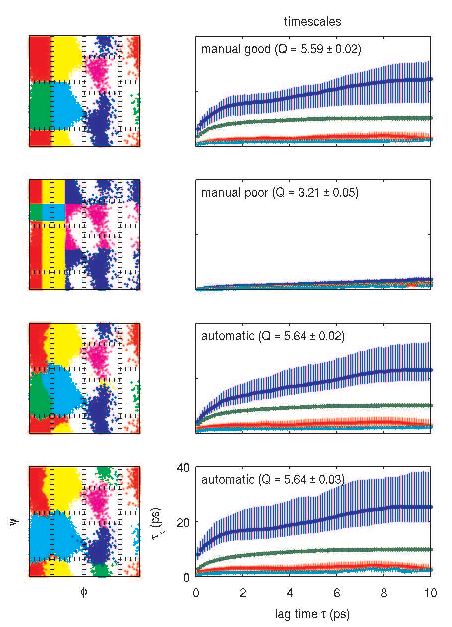
\includegraphics{chapters/automatic-state-decomposition/figures/alanine-dipeptide/alanine-dipeptide-comparison-manual-automatic.pdf}}
  \end{center}
  \caption{{\bf Comparison of manual and automatic state decompositions for alanine dipeptide.}  
  The left panels depict state partitionings, and the right panels the associated timescales (in picoseconds) as a function of lag time with uncertainties shown, as estimated from the procedure described in Section \ref{automatic:section:methods:validation}.
  Top two panels: Manual ``good'' or ``gold standard'' state decomposition from Ref.\ \cite{chodera:mms:2006} and manual ``poor'' state decomposition, where the state boundaries are grossly distorted so as to include internal kinetic barriers within the states.
  Bottom two panels: Two nearly-equivalent partitionings obtained from the automatic state decomposition algorithm.
  }
  \label{automatic:figure:alanine-dipeptide-manual-vs-automatic}
\end{figure}

The results of the automatic state decomposition algorithm applied to this reduced dataset can be seen in Figure \ref{automatic:figure:alanine-dipeptide-manual-vs-automatic}, in comparison with the ``gold standard'' manual state decomposition from Ref.\ \cite{chodera:mms:2006} and a ``poor'' manual decomposition that is expected to fail to reproduce kinetics well because its states include internal kinetic barriers\footnote{The poor partitioning was defined as follows: (1) $\phi \in [(179,-135]$, $\psi \in (98,48]$; (2) $\phi \in (-135,-60]$, $\psi \in (98,48]$; (3) $\phi \in (179,-135]$, $\psi \in (48,98]$; (4) $\phi \in (-135,-60]$, $\psi \in (48,98]$; (5) $\phi \in (-60,179]$, $\psi \in (98,-45]$; (6) $\phi \in (-60,179]$, $\psi \in (-45,98]$.  Specified intervals denote intervals on the torus, which is continuous from -180 to +180.  All torsions are specified in degrees.}.
Independent applications of the automatic method were observed to yield two distinct decompositions with metastabilities within statistical uncertainty, both of which slightly exceeded the metastability of the manual decomposition (Figure \ref{automatic:figure:alanine-dipeptide-manual-vs-automatic}, bottom two plots).
In the automatic decomposition with slightly larger metastability, six states in the same general locations as the manual ``gold standard'' decomposition are observed, though the boundaries are somewhat perturbed.
However, the timescales as a function of lag time are not significantly different from those of the manual ``gold standard'' decomposition  (Figure \ref{automatic:figure:alanine-dipeptide-manual-vs-automatic}, right) .
In the other automatic decomposition with nearly equal metastability, states 3 and 4 of the manual decomposition (numbering given in Figure \ref{automatic:figure:alanine-dipeptide-2d-pmf}) have been merged into a single state, and state 5 of the manual decomposition has been fragmented into two states.
Despite this, the timescales as a function of lag time again appear to be statistically indistinguishable from those of the ``gold standard'', suggesting that this model may have equal utility.
This suggests that the phenomenological rates may not be very sensitive to the exact choice of state boundaries after the Markov time, as recrossings will have been suppressed by this time.
The fact that this lumping does not disrupt the behavior of the model substantially is not altogether surprising, because the barrier separating states 3 and 4 is rather small, and these states act like a single state even on timescales of a few picoseconds or greater.
In contrast, the ``poor'' decomposition has extremely short timescales which do not appear to level off over the course of 10 ps.

\begin{figure}[tb]
  \begin{center}
    \resizebox{3.375in}{!}{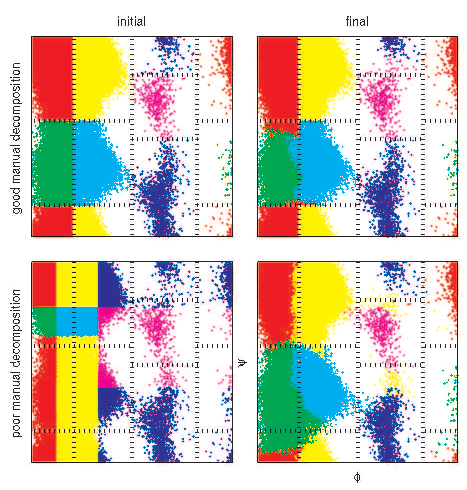
\includegraphics{chapters/automatic-state-decomposition/figures/alanine-dipeptide/alanine-dipeptide-comparison-initial-final.pdf}}  
  \end{center}
  \caption{{\bf Stability and recovery of optimal state decomposition for alanine dipeptide.}
  Top: Ten cycles of automatic state decomposition applied to a ``good'' manual partitioning (left) to yield an automatic partitioning (right).
  Bottom: Ten cycles of automatic state decomposition applied to a ``poor'' manual partitioning (left) to yield an automatic partitioning (right).
  }
  \label{automatic:figure:alanine-dipeptide-decomposition-stability}
\end{figure}

To examine the ability of the algorithm to recover optimal partitionings, the automatic state decomposition algorithm was applied to both the ``gold standard'' and ``poor'' manual decompositions (Figure \ref{automatic:figure:alanine-dipeptide-decomposition-stability}) to see whether these partitionings would be maintained over the course of subsequent iterations.
Ten iterations were conducted, with each macrostate split to ten microstates in the first iteration, rather than the entire configuration space being split into 100 states.
In both cases, the algorithm converged to nearly equivalent partitionings after ten iterations (Figure \ref{automatic:figure:alanine-dipeptide-decomposition-stability}), as verified by examination of the converged timescales (data not shown).
This suggests the method yields partitionings that are relatively stable and optimal.

From the ``poor'' manual decomposition, however, a number of conformations in manual states 5 and 6 are incorrectly grouped with state 2, though this did not significantly affect the timescales.
Further investigation showed that the algorithm never split these conformations from state 2, partly due to their comprising only 1 \% of the population of the state.
Splitting each macrostate into more microstates should alleviate this problem.

\subsection{The F$_s$ helical peptide.}
\label{automatic:applications:helix}

% TODO:

% TWO-COLUMN TABLE OF STATES FOR ALPHA HELIX
\newcommand*{\DOT}{.}
\newcommand{\colpdbwidth}{0.75in}
\newcommand{\pdbfigcol}[1]{\parbox{\colpdbwidth}{\includegraphics[width=\colpdbwidth]{#1}}}
\newcommand{\pdbimg}[1]{\pdbfigcol{chapters/automatic-state-decomposition/figures/alpha-helix/state-pdbs/10\DOT ensemble-merged-#1.png}}
\begin{table*}[tb]
\caption{{\bf Macrostates from a 20-state state decomposition of the F$_s$ helical peptide.}  The backbone is depicted in alpha carbon trace, and arginine sidechains are shown in blue (Arg10), magenta (Arg15), and green (Arg20) for clarity.}
\label{automatic:table:helix-states}
\begin{center}
\begin{tabular}{ccccccccc}
\hline
state & 1 & 2 & 3 & 4 & 5\\
& \pdbimg{143215} & \pdbimg{116359} & \pdbimg{509002} & \pdbimg{344096} & \pdbimg{118439} \\
members & 358 712 & 98 222 & 46 921 & 22 559 & 22 367 \\
$\tau_\mathrm{ac}$ (ns) & 3.1 & 0.9 & 1.4 & 0.6 & 4.0 \\
\hline
state & 6 & 7 & 8 & 9 & 10 \\
&  \pdbimg{544652} & \pdbimg{189995} & \pdbimg{439117} & \pdbimg{514253} & \pdbimg{607324} \\
members & 15 859 & 11 975 & 11 053 & 11 024 \\
$\tau_\mathrm{ac}$ (ns) & 1.3 & 1.6 & 2.2 & 2.0 \\
\hline
state  & 11 & 12 & 13 & 14 & 15 \\
 & \pdbimg{532115} & \pdbimg{16278} & \pdbimg{618465} & \pdbimg{438247} & \pdbimg{509683} \\
members & 7 976 & 7 808 & 7 771 & 5 978 & 5 626 \\
$\tau_\mathrm{ac}$ (ns) & 2.2 & 1.2 & 1.6 & 11.3 & 2.3 \\
\hline
state  & 16 & 17 & 18 & 19 & 20 \\
& \pdbimg{257470} & \pdbimg{348373} & \pdbimg{503295} & \pdbimg{484545} & \pdbimg{596094} \\
members & 1 856 & 955 & 531 & 525 & 490 \\
$\tau_\mathrm{ac}$ (ns) & 5.0 & 10.3 & 47.0 & 29.1 & 15.2 \\
\hline
\end{tabular}
\end{center}
\end{table*}

To illustrate behavior of the automatic state decomposition method on a larger peptide system with fast kinetics, we applied it to the 21-residue helix-forming F$_s$ peptide, which has been studied extensively both experimentally \cite{lockhart:science:1992,lockhart:science:1993,williams:biochem:1996,eaton:biochem:1997,lednev:jacs:2001} and computationally \cite{garcia:2002a,duan:jpcb:2004,sorin:2005a,sorin:2005b}.
Since helix formation occurs on the nanosecond timescale, Sorin \emph{et al.}\ were able to reach equilibrium from both helix and coil conformations and observe equilibrium conformational dynamics using ensembles of molecular dynamics trajectories on the distributed computing platform Folding@Home \cite{sorin:2005b}.
Two sets of 1000 trajectories at 302 K of varying length of the capped F$_s$ peptide (sequence Ace-A$_5$[AAARA]$_3$A-Nme), one set initiated from an ideal helix and another from a random coil, were obtained from Sorin \emph{et al.}\cite{sorin:2005b}; details of the simulation protocol are available therein.
The first 40 ns of each trajectory, a conservative overestimate of the time to reach equilibrium from either helix or coil, was discarded, and the two sets of trajectories combined to yield a total of 1689 trajectories varying in length from 10 ns to 95 ns with a sampling interval of 100 ps.
In total, this equilibrium dataset contained nearly 65 $\mu$s of simulation data in 642 604 conformations.
The peptide was modeled using the AMBER-99$\phi$ forcefield \cite{AMBER-parm99,sorin:2005b} and solvated in TIP3P water \cite{jorgensen:1983a}.
Though the Berendsen weak-coupling scheme \cite{berendsen:1984a} was employed for thermal and pressure control\footnote{We note that thermal and pressure control, by design, modulate the velocities of molecules in the system, which may have a nonphysical effect on dynamics.  In this particular application, however, we are only comparing our analysis with the original simulation data, rather than directly with experiment.}, we presume the trajectories still obey microscopic reversibility when only the coordinates of the macromolecular solute are considered for the purposes of computing transition probabilities.

We performed automatic state decomposition on this dataset to generate a set of 20 macrostates through 10 iterations of splitting and lumping.
In the first iteration, the sampled region of conformation space was split into 400 microstates.
In subsequent iterations, each macrostate was split into 50 microstates (or, if the expected microstate size would fall below 500 configurations, a number of microstates chosen to ensure the expected microstate size would remain above this threshold). 

Automatic state decomposition produced a structurally diverse set of states (Table \ref{automatic:table:helix-states}), ranging in size from over 350 000 members to 500 members, with the majority containing from 5 000 to 20 000 members.  
The states include a large extended helix/coil state (state 1 of Table \ref{automatic:table:helix-states}), consisting of slightly over half the total conformations in the dataset; a pure helix state (state 15); a number of helix/coil states which are bent in half to different degrees to form tertiary contacts (states 2--14); and a number of smaller helical states which are bent into circles to form tertiary interactions (states 16--20). 
A previous analysis of this data clustered conformations into states based on dissimilarity in various order parameters: the number of helical residues, number of helical segments (stretches of helical residues), length of the longest helical segment, and radius of gyration \cite{sorin:2005b}.
We compared the macrostates generated by the automatic algorithm with these clusters, and found that while some states are similar, namely the bi-nucleated helices of different sizes, most were quite different.
The most significant difference was the grouping of helix and coil conformations into a single macrostate in the lumping phase of the automatic algorithm; the order parameter-based clustering kept helix and coil states distinct \cite{sorin:2005b}.
When examining individual trajectories, we noticed conformations would rapidly flicker between helices and coils between consecutive frames of the trajectory, suggesting that their rapid interconversion justifies their lumping into a single macrostate.
Additionally, the clustering based on helical order parameters was unable to distinguish certain structures that involved tertiary contacts, such as the bent and circular helical states.
Interestingly, a previous study employing the related AMBER parm03 forcefield \cite{duan:2003a} identified similar configurations to those noted by the automatic state decomposition, terming these states helix (corresponding to our state 1), helix-turn-helix, adjusted helix-turn-helix, helix-wind-helix, globular helix (states 16--20), and helix tail (state 15) \cite{duan:jpcb:2004}.
% JDC: Maybe add our state definitions?

%  list of the states, we won't actually include this, but just for reference at this point:
%	143215 - extended helix/coil with 359K members, 116359 - bent helix/coil with 98K members, 509002 - expanded helix-turn-helix with 47K members, 344096 - helix/coil with kink at last turn with 23K members, 118439 - helix-turn-helix with twist with 22K members, 544652 - helix-turn-helix with 16K members, 189995 - uneven helix-turn-helix with twist with 12K members, 439117 - helix-turn-helix with 11K members, 514253 - uneven helix-turn-helix with 11K members, 607324 - uneven twisty helix-turn-helix with 8K members, 532115 - star-like helix-turn-helix with 8K members, 16278 - uneven helix-turn-helix with 8K members, 618465 - helix-turn-helix with kink at bend - 6K members, 438247 - helix-turn-helix with slight twist with 6K members, 509683 - extended helix with 4K members, 257470 - star-like with planar tails with 2K members, 348373 - star with 1K members, 503295 - helix-turn-helix with twist with 500 members, 484545 - star-like with 500 members, and 596094 - star-like with 500 members.

% TIMESCALES PLOT
\begin{figure}[tb]
  \begin{center}
    \resizebox{3.375in}{!}{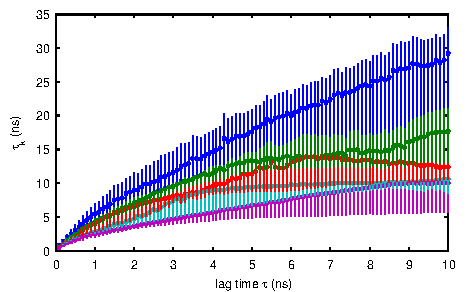
\includegraphics{chapters/automatic-state-decomposition/figures/Fs-peptide/Fs-timescales.pdf}}    
  \end{center}
  \caption{{\bf Implied timescales of the F$_s$ peptide as a function of lag time for 20-state automatic state decomposition.} 
   The five longest timescales are shown.  
   Circles represent the maximum likelihood estimate, and vertical bars depict 68\% symmetric confidence intervals about the mean.
   Note the timescales associated with two processes appear to cross, but are here colored and uncertainties are estimated with bootstrapping by ordering them by rank.
   This may cause the uncertainties depicted here to be an underestimate of the true uncertainties of each process.
  }
  \label{automatic:figure:fs-peptide-timescales}
\end{figure}

We then examined the implied timescales as a function of lag time (Figure \ref{automatic:figure:fs-peptide-timescales}).
%In the first iteration of microstates, all the largest timescales increased with lag time, with the longest timescale rising from 2.5 ns at 500 ps lag time to 10 ns at 10 ns lag time.  
%The timescales between the split microstates and lumped macrostates were extremely similar through all the iterations.  
%By the end of the tenth iteration, many of the timescales leveled off by a lag time of 3-5ns.  However, some timescales did continue to rise over the range of lag times -- a signature of non-Markovian behavior.  
%In particular, the longest timescale rose from 3 ns at 500 ps lag time to 30 ns at 10 ns lag time. [FIGURE - show the lifetimes versus lag time at iteration 10-merged]
Lumping appeared to preserve the longest timescales found in the microstate transition matrix (data not shown), indicating that our lumping scheme had been successful in identifying a nondestructive lumping into kinetically metastable states at each iteration.
%Over the course of 10 iterations, the longest timescale (as assessed with a lag time of 10 ns) increased from 10 to 30 ns, suggesting that the iterative refinement was actually improving the quality of the state decomposition.
% JDC: Can we also give the metastabilities vs iteration?  That might be a nice way to summarize improvement.
% NS: I like that -- I'm going to report it at 100 ps since that's the lag time for which we're actually maximizing it
% NS: 1st iteration -- lag time of 100ps, Q = 12.5358, lag time of 10 ns, Q = 2.2949
% NS: 10th iteration -- lag time of 100ps, Q = 14.5024, lag time of 10 ns, Q = 4.3512
% NS added:
Over the course of 10 iterations, the metastability (as optimized with a lag time of 100 ps) increased from $12.5 \pm 0.3$ to $14.5 \pm 0.1$, suggesting that the iterative refinement was actually improving the quality of the state decomposition.
% NS deleted since this doesn't really seem true when looking at the figure.
%On the first iteration, the longest timescales increase nearly linearly with lag time, while on the last iteration, most timescales became stable by a lag time of 10 ns, suggesting that Markovian behavior had been achieved.
On the first iteration, the longest timescales increase nearly linearly with lag time, while on the last iteration, some of the longest timescales become stable by a lag time of 4 -- 5 ns, suggesting Markovian behavior for some of the processes.

Using the interpretation of eigenvector components in terms of aggregate modes described in Section \ref{automatic:section:theory:markov-model-introduction}, the longest timescale was found to correspond to movement between the extended helix/coil state (state 1) and one of the twisted helix-turn-helix states (state 18) with only 500 members.  
We found, however, that state 18 appeared a small number of times in thirty trajectories, and over 450 times in a single trajectory.
% JDC: Nina -- is this right?
% NS: Yup, I wrote a script to count the number of conformations per trajectory for each state.  This was a particularly long trajectory, which is why I think we initially thought it was in more than one.
Further examination revealed that conformations belonging to this state were almost exclusively adjacent to conformations belonging to state 5, and structural comparison of conformations of these two states showed they were strikingly similar.
This suggests that slight conformational differences between conformations in states 18 and 5 allowed the $K$-medoid clustering algorithm to partition between these states in a splitting step, and since state 18 was mainly isolated in a single trajectory, its self-transition probability was maximized by \emph{not} lumping it with state 5, even though the two behaved in a similar kinetic fashion.
Indeed, when we manually lump states 18 and 5, the longest timescale, corresponding to transitions involving state 18, disappears, but the remaining timescales are all preserved (data not shown).
% JDC: Do we want to comment on the importance of having many effectively independent trajectory segments passing through the same state?
% NS: I feel this is covered pretty well in the end when we talk about the statistical inefficiency, no?

A second potential cause of the increase with lag time observed 
% NS changed: I feel we've sufficiently explained away the rise in the longest timescale and are now trying to explain the rise in the other timescales.
% in the longest timescale 
in some of the other long timescales
may be due to the finite length of trajectories.
If the state is long-lived, and occurs near the trajectory beginning or end, then it can be seen that the estimated self-transition probability $T_{ii}$ increases as a function of lag time.
This effect is most pronounced when a state occurs in very few trajectories, and appears to be mitigated when the state occurs in many trajectories at random times within the trajectory.
%We believe a second cause of the rising timescales with lag time is that the finite length of the trajectories causes end effects with increasing lag time, and these end effects are more pronounced in states with less sampling. % Fix me
% JDC: Elaborate on this.
          
In order to determine which states are poorly characterized, we estimated the number of statistically independent visits to each macrostate.
Since sequential samples from a single trajectory are temporally correlated, we computed the integrated autocorrelation time \cite{swope:1982a,janke:2002a} $\tau_{\mathrm{ac},i}$ for each macrostate $i$.
% NS changed so two sentences don't start "in the absence of"
% In the absence of statistical uncertainty, 
Ignoring statistical uncertainty, this correlation time is an upper bound on the equilibration time within a state; long-lived states will necessarily have long autocorrelation times, but trajectories trapped within them may contain many uncorrelated samples if the internal equilibration time is short.
In the absence of a convenient way to quantify the internal equilibration time for each state\footnote{There is some indication that consideration of restrictions of Markov chains to these macrostates may facilitate the computation of the internal equilibration time \cite{meerbach:2004a}.}, the autocorrelation time provides a better estimate of the appropriate timescale than the time to reach global equilibrium $\tau_{\mathrm{eq}}$.
%In order to determine which states may be poorly characterized, we attempted to estimate the number of statistically independent visits to each macrostate.
%We calculated the normalized fluctuation autocorrelation function $C_{ii}(t)$ for each state $i$
%\begin{eqnarray}
%C_{ii}(t) &=& \frac{\expect{\chi_i(0) \chi_i(t)} - \expect{\chi_i}^2}{\expect{\chi_i^2} - \expect{\chi_i}^2} \\
%           &=& \frac{T_{ii}(t) - p_i}{1 - p_i} .
%\end{eqnarray}
%where $T_{ii}(t)$ is the diagonal element of the transition probability matrix at time $t$ and $p_i$ is the equilibrium probability of state $i$.
%Expectations were estimated as averages over all trajectories, employing both stationarity and time-reversibility.
%This correlation function assumes the value of unity at $t = 0$, and decays to zero as the state occupied by the trajectories becomes decorrelated with this initial state occupation.
%The integrated autocorrelation time $\tau_i$ is a measure of the time required for decorrelation, and is given by
%\begin{eqnarray}
%\tau_i = \sum_{t=1}^T \left( 1-\frac{t}{T} \right) C_{ii}(t) . \label{automatic:equation:integrated-autocorrelation-time}
%\end{eqnarray}
As the correlation functions became statistically unreliable at times larger than 10 ns, a least squares linear fit to the log of the computed correlation function over the first 10 ns was used to estimate the tail at times greater than 10 ns, and this combined correlation function 
% NS added
was
integrated to obtain the autocorrelation time.
The effective number of independent samples for each state was then estimated by summing the number of independent samples from each trajectory (which are assumed independent), where the effective number of independent samples of state $i$ from trajectory $n$ is computed as  $N^\mathrm{eff}_{ni} \approx \min\{ 1, N_{ni} / g_i \}$, where $N_{ni}$ is the number of configurations from trajectory $n$ in state $i$, and $g_i = 1 + 2 \tau_{\mathrm{ac},i}$ is the statistical inefficiency of state $i$.

Computed state autocorrelation times are given in Table \ref{automatic:table:helix-states}.
For many states, the correlation time was 1 -- 2 ns, giving thousands of independent samples; however, for five states, including the four which were involved in the four longest timescales, the correlation times were between 10 and 50 ns, suggesting that the dataset contained less than 
% NS changed: If we give one independent sample per trajectory, the last four states have 67, 30, 26, and 47 independent samples respectively.  The other state with large correlation time (13) has 256 independent samples
50
%ten 
independent samples of these states.
Currently, in the automatic state decomposition algorithm, we try to reduce the statistical uncertainty in the transition matrix by limiting the expected population of each state to be greater than some minimum number of configurations.
Since the conformations appearing within some states may be highly correlated, the number of conformations within a state is not the best measure of how statistically well-determined its transition elements are; instead, it may be advantageous to place a lower limit on the effective number of independent visits to each state, which is far less than the number of configurations it contains.
Alternatively, it may be necessary to ensure better characterization of these states by conducting additional simulations from them, provided the equilibrium transition probabilities can still be computed.

% TIME EVOLUTION PLOT
\begin{figure}[tb]
  \begin{center}
    \resizebox{3.375in}{!}{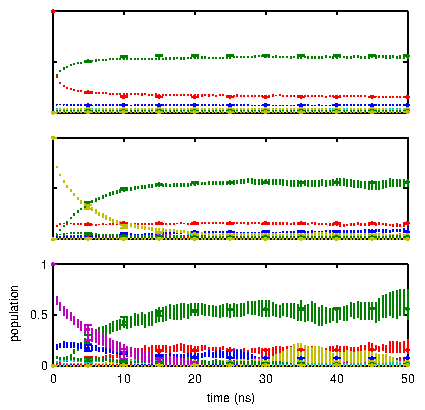
\includegraphics{chapters/automatic-state-decomposition/figures/Fs-peptide/fs-time-evolution.pdf}}    
  \end{center}
  \caption{{\bf Reproduction of observed state population evolution by Markov model for the F$_s$ peptide.} 
  The time evolution of the Markov model constructed from the 5 ns lag time transition matrix is shown by the filled circles with flat error bars, which denote the 68\% confidence interval from realizations of a bootstrap sample of 40 transition matrices computed from a 5 ns lag time.
  Vertical bars without flat ends denote the 68\% asymmetric confidence interval for the probability of finding the system in the 20 macrostates a given time after initial preparation in a specific state.
  The system was originally prepared in state 2 (top, red), 13 (middle, yellow), or 19 (bottom, purple).
  The most populous states are colored green (state 1), red (state 2), and blue (state 3).
  }
  \label{automatic:figure:fs-time-evolution}
\end{figure}

%Because of the difficulties described above, the models we were able to build for the F$_s$ peptide were not Markovian over reasonable timescales.
%However, our timescales corresponding to motion between well determined states, such as the extended helix/coil and bent helix/coil seem to be on the order of 5 -- 10 ns, which are not unreasonable given the extremely conservative estimate of full equilibration from an extremely biased starting conformation of 40 ns \cite{sorin:2005b}.
%We hope future versions of this algorithm will give shorter Markov times and shed more light on the kinetics of the F$_s$ peptide.
% JDC: COmmented this out.

We constructed a Markov model from the transition matrix estimated at a 5 ns lag time, where some (though apparently not all) of the timescales appear to have stabilized.
Repeated application of this transition matrix to an initial probability distribution can be compared to the transition probabilities at longer lag times estimated directly from the data to assess how well the model reproduces the observed kinetics.
The time evolution of probability density out of three states (state 2, a populous state; state 13, a moderately populated state; and state 19, a sparsely populated state) over the course of 50 ns is shown in Figure \ref{automatic:figure:fs-time-evolution}.
The Markov model appears to do a very reasonable job of predicting the time evolution of the system to within statistical uncertainty over many times longer than the lag time it was constructed for.
In fact, the time evolution was well-modeled for evolution out of nearly all states, except for state 13, for which dynamics seemed to be particularly poorly reproduced.
This state has a particularly long correlation time, and many trajectories seem to contain only a single configuration that is part of this state, suggesting its boundaries are simply poorly resolved.
Regardless, the time evolution is generally well-modeled for this system.

% Left from previous version, I don't think we need to do this -- Discuss whether the "star-like" trap states are artifacts of the sampling, force field, or actual states that are hard to observe experimentally.

% Old part left-over from previous version.  I don't think we can actually do this since the Markov time is too high compared with the overall equilibration time of the system.
    %Comparison with simulation data:
    %We eliminated the first 40 ns of simulation data, so the starting conformation of the trajectories was taken from an equilibrium distribution.
    %We selected those trajectories whose starting conformation was in a particular state, and plotted the state populations with time, for those trajectories.
    %We also calculated the state populations with time, given by the model propagated from a population of one of the given states.
    %(FIGURES of the comparison starting from different states)


\subsection{The trpzip2 $\beta$-peptide.}
\label{automatic:applications:hairpin}

\begin{figure*}[tb]
  \begin{center}
    \resizebox{\textwidth}{!}{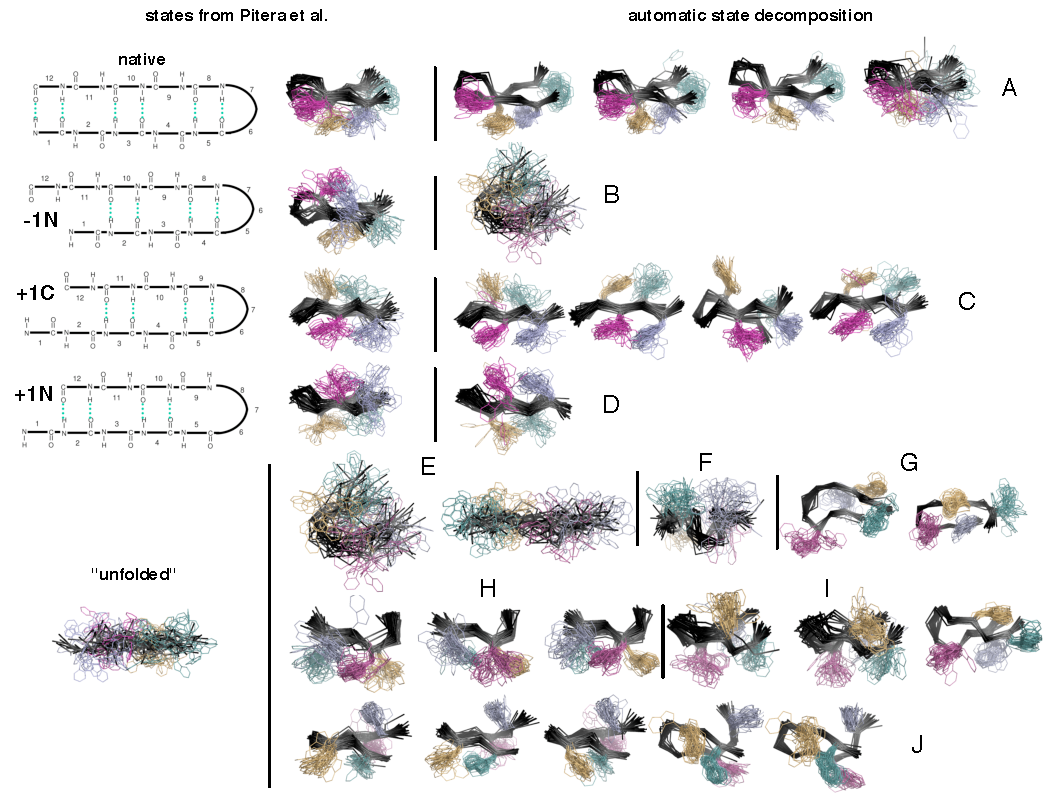
\includegraphics{chapters/automatic-state-decomposition/figures/trpzip2/comparison-with-reptated-states.pdf}}    
  \end{center}
  \caption{{\bf Comparison of some trpzip2 macrostates found by automatic state decomposition with misregistered hydrogen bonding states identified in a previous study.}  
  Left: The five hydrogen bonding patterns enumerated in Pitera \emph{et al.\ } \cite{pitera:2006a} that occurred in sufficient numbers in the subsampled trpzip2 dataset used here, with representative conformational ensembles.  
  Right: A selection of macrostates discovered by automatic state decomposition that the contain the largest numbers of hydrogen bonding pattern states.  
  The backbone is depicted in alpha carbon trace, and tryptophan sidechains are shown in light blue (Trp2), orange (Trp4), magenta (Trp9), and teal (Trp11).
  A complete set of macrostates obtained from the 40-state decomposition of the trpzip2 dataset is available as Supplementary Information.
  }
  \label{automatic:figure:trpzip2-states}
\end{figure*}

\begin{figure}[tbp]
  \begin{center}
    \resizebox{3.375in}{!}{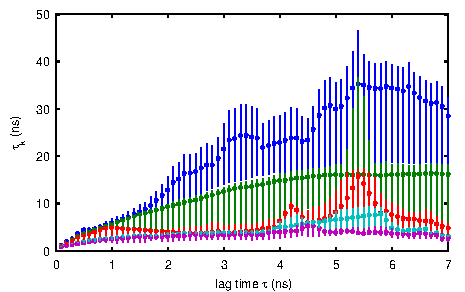
\includegraphics{chapters/automatic-state-decomposition/figures/trpzip2/trpzip2-timescales.pdf}}    
  \end{center}
  \caption{{\bf Implied timescales of trpzip2 as a function of lag time for 40-state automatic state decomposition.}  The five longest timescales are show.  Vertical bars depict 68\% confidence intervals.}
  \label{automatic:figure:trpzip2-timescales}
\end{figure}

As an illustration of the application of the state decomposition algorithm to a system with complex kinetics implying the existence of multiple metastable states \cite{yang:2004c}, we considered the engineered 12-residue $\beta$-peptide trpzip2 \cite{cochran:2001a}.
A set of 323 10 ns constant-energy, constant-volume simulations of the unblocked peptide\footnote{Note that the peptide studied experimentally in Refs. \cite{cochran:2001a} and \cite{yang:2004c} was synthesized with an amidated C-terminus, whereas the termini of the simulated peptide in the dataset considered here were left zwitterionic.} simulated using the AMBER parm96 forcefield \cite{AMBER-parm96} in TIP3P water \cite{jorgensen:1983a} was obtained from Pitera et al.\ \cite{pitera:2006a}; 
details of the simulation protocol are provided therein.
The trajectories were initiated from an equilibrium sampling of configurations at 425 K, a temperature high enough to observe repeated unfolding and refolding events at equilibrium.
Configurations were sampled every 10 ps, giving a total of 3.23 $\mu$s of data in 323 000 configurations.

The automatic state decomposition method was applied to obtain a set of 40 macrostates in 10 iterations of splitting and lumping.
In the first iteration, the conformations were split into 400 microstates, and in subsequent iterations, as described in Section \ref{automatic:section:methods:implementation}.

Figure \ref{automatic:figure:trpzip2-states} depicts some of the final set of 40 macrostates compared with a set of states produced by consideration of backbone hydrogen bonding patterns in a previous study by Pitera \emph{et al.} \cite{pitera:2006a}.
(The complete set of macrostates is shown in a figure included as Supplementary Information.)
As the trajectories considered here were resampled to 10 ps intervals (rather than 1 ps in Ref. \cite{pitera:2006a}) we found less than five examples of the +2 and -2 hydrogen bonding states identified in Ref. \cite{pitera:2006a}, and therefore do not include them in the comparison.
The automatic state decomposition method recovers states corresponding to the native, +1C, and +1N hydrogen bonding patterns, and often further separates conformations based on the packing of the tryptophan sidechains (Figure \ref{automatic:figure:trpzip2-states}, A, C, D).
However, the -1N hydrogen bonding pattern is not further resolved, and instead is grouped into a state of mostly disordered hairpins; further examination is necessary to determine whether the algorithm simply failed to resolve this state or if the state is simply not long-lived.
% JDC: Nina will check integrated correlation time of this state.
% NS: John, I *think* I know the correspondence between jed's state numbers and the hydrogen bonding pattern, but I enumerated it below just in case
% NS: Since some of the states were so small, they had zero count for their self-transition probability at some lag times.  This caused imaginary values when I took the log to estimate the exponential fit, so I didn't include them in the exponential fit, and used the fit in the correlation time calculation instead of the real value.  This did not change any of the helix correlation times since ever had zero counts.
% NS: state 1 (native) - tau = 1713.3 (in 10ps) = (17 ns?)
% NS: state 2 (unfolded) - tau = 1414.8 (in 10ps) = 14 ns
% NS: state 3 -- no examples
% NS: state 4 (-1N) - tau - 91.6 (in 10ps) = .9 ns 
% NS: state 5 (+1C) - tau - 235.8 = 2.4 ns
% NS: state 6 (+1N) - tau - 817.6 = 8.2 ns
% NS: state 7 (too unreliable)
% NS: state 8 (too unreliable)
In addition to recovering most of the manually identified misregistered states, the algorithm was also able to greatly resolve the state labeled as ``unfolded'' in Pitera \emph{et al.} (in that it did not conform to any of the enumerated hydrogen bonding patterns) into substates which exhibit considerable structure (E--J).
Some of these kinetically resolved states have distinct hydrogen bonding patterns, such as where both strands are rotated (H), causing the tryptophan sidechains to appear on the opposite face, or where the misregistration is greater than two residues (G, J). 
% JDC: Check that these letters are right?
% NS: I don't know if J has large misregistration, is it easy to calculate hydrogen bonding patterns for a few conformations, since I have a hard time telling by eye.
This demonstrates the utility of the method in identifying additional kinetically relevant states that were not initially part of the experimental hypothesis space.

Figure \ref{automatic:figure:trpzip2-timescales} depicts the implied timescales of the kinetic model as a function of lag time.
The longest timescale ranges between 25 and 35 ns and appears to stabilize over the range of lag times considered, though the uncertainty is quite large.
Eigenvector analysis (described in Sec. \ref{automatic:section:theory:markov-model-introduction}) shows that this timescale corresponds to transitions between the unfolded and disordered hairpin states (E) and the hairpin with both strands rotated (H).
% JDC: Double-check?
% NS: I think that is right
The states labeled H together totaled 935 conformations, but appeared in only 13 trajectories, with over 95\% of the conformations appearing in a single trajectory.
% JDC: Which states?
% NS: The "H" states
Correlation time analysis (Sec. \ref{automatic:applications:helix}) suggests there are less than 10 independent samples for each of the three states, so proper resolution of this timescale would require more data.
% JDC: Fill in number.
% NS: There were also problems with the exponential fit since some states went to 1 at long lag times, causing the corr time to go to infinity.  I eglected these tau's as well.
% NS: State 10126 - tau = 115.3 (in 10 ps) = 1.2 ns, g = 232, 216 members --> number of trajectories = 6  
% NS: State 10503 - tau = 312.4 (in 10 ps) = 3.1 ns, g = 626, 446 members --> number of trajectories = 9
% NS: State 10772 - tau = 273.0 (in 10 ps) = 2.7 ns, g = 547, 273 members --> number of trajectories = 4
The second longest timescale grows to about 15 ns and levels off by around 4 ns, and corresponds to transitions between the unfolded and disordered hairpin states (E) and the 
% NS changed
% four states corresponding to \emph{native} in Figure \ref{automatic:figure:trpzip2-states}.
native backbone states (A).
The states involved in this transition are much better characterized, with a total of over 25 000 conformations appearing in over half the trajectories.
The next three longest timescales were all between 3 and 4 ns and correspond to movement between the unfolded state (E) and various sets of misregistered states, namely
%row 3 of the unfolded state, row 4 of the unfolded state, and the +1C state.
% NS deleted:
% reptated states G and I, and the +1C state (state C).
the newly identified misregistered states I and J, and the +1C state (C).
% JDC: Double-check these!
Unfortunately, these timescales are on the order of the Markov time for the whole system, so it is difficult to characterize these transitions well.
% JDC: Elaborate!

%\begin{itemize}
%%  \item Timescales
%%  \begin{itemize}
%%    \item Timescales (except for slowest) level off around 3 ns, suggesting a Markov time (internal equilibration time) of 3 ns.
%%    \item Slowest timescale at this point is unfolding/misfolding of bent/inside-out/all trp on back face hairpin.  (Two such states: 10042 and 10351.)  Timescale might be as long as 40 ns, but very low population state, and very little confidence in estimated timescale.  Can make a statement like ``90\% of snapshots in the state came from one or two trajectories''.
%%    \item Next-slowest timescale is much more robust, levels off, more well-determined.  Mostly transitions between folded unfolded/extended/collapsed hairpin with the two folded/native states. 20 ns timescale.
%%    \item Should we look up loosely-packed to well-packed native hairpin transition? - occurs on 1-3 ns timescale at 5ns lagtime
%%    \item Big gap in timescales, next slowest timescales correspond to unfolded to misfolded/reptated transitions, with timescales around 5 ns.  Can identify what some of these are.  
%%    \item Next-slowest timescale has one reptation, but sidechains of different member states are in different rotameric states.
%%  \end{itemize}
%  \item Time-evolution of model?
%  \item Main messages.
%   \begin{itemize}
%    \item We can pick up same states as Jed found manually, but done automatically.
%    \item Folding mechanism is same as Jed/Imran found: no reptation, misfolded states must unfold.
%    \item Slowest timescale may be unfolding from trap, but not enough data to be sure.  Next-slowest is folding.  Gap in timescales before faster aggregate timescales.
%   \end{itemize}
%   \item Something about how resulting model has some timescales faster than lag time, and might need to lump these out?
%   \item Could we compare these states with states we get from K-means, which are not kinetically meaningful?
%\end{itemize}

%% DISCUSSION %%%%%%%%%%%%%%%%%%%%%%%%%%%%%%%%%%%%%%%%%%%%%%%%%%%%%%%%%%%%%%%%%%%%

\section{Discussion}
\label{automatic:section:discussion}

% TODO:
% - Add a note about large uncertainties in timescales plot.  What would we need to reduce these?  How do these uncertainties compare to uncertainties in experimental kinetic measurements?

Markov models are expected to be effective and efficient ways to statistically summarize information about the pathways (mechanism) and timescales for heterogeneous biomolecular processes such as protein folding.  
The great challenge is in defining an appropriate state space.  
Here, we have presented a new algorithm for automatically generating a set of configurational states that is appropriate for describing peptide conformational dynamics in terms of a Markov model, though we expect it to be applicable to macromolecular dynamics in general.  
The algorithm uses molecular dynamics simulations as input, and generates the state definitions using information about the temporal order of conformations seen in the trajectories.
The importance of having an automatic algorithm, \emph{i.e.}, one that requires little or no human intervention, is that without it, human bias may inadvertently produce incorrect interpretations of the mechanism of conformational change by imposing a particular view on the simulation data.
Additionally, molecular simulation datasets are becoming so large and complex that effectively summarizing the data or extracting insight becomes increasingly impractical unless the experimenter analyzes the data with a specific hypothesis in mind.
Construction of a Markov model, however, allows for a ``hypothesis-free'' investigation of conformational dynamics, provided that the state space is sufficiently well sampled.

Our algorithm is based on the availability of large numbers of molecular dynamics simulations of appropriate simulation length such as might be generated by a supercomputer or a large (possibly distributed) cluster.  
Current technology allows for the production of thousands of simulations that can be tens of nanoseconds in length, hundreds of trajectories of up to hundreds of nanoseconds in length, or dozens that are on the order of a microsecond in length.
Since our goal has been to develop Markov models that accurately characterize the time evolution of ensembles of macromolecules over experimental timescales (that can range from microseconds to milliseconds) from short simulations of single molecules, our approach places strong emphasis on the longest timescales observed in molecular simulations.
For example, recognizing that ill-formed states often result in artificially shortened timescales, we sought to find states that maximize the timescales implied by their corresponding transition matrix for a particular choice of lag time and number of states.  
This resulted in the maximization of the metastability as a computationally convenient surrogate for minimizing the internal equilibration time $\tau_{\mathrm{int}}$.
%use of the trace of the transition matrix as a figure of merit for the decomposition, a computationally convenient surrogate for the sum of state lifetimes for the entire decomposition.  
%We also seek states for which the implied timescales are stable with respect to the lag time used to construct the transition matrix, and, in particular, the decomposition where this stability is achieved at the smallest possible lag time.  
%%This produces states of greater utility in that they are also capable of describing some of the faster processes, but usually it is more difficult to achieve this stability for the longer time scales.
%% JDC: Removed this because we weren't sure what it meant.


Nonetheless, for the three data sets to which we have applied the method, there have been a number of important successes.  
For alanine dipeptide, the algorithm discovered a distinct manifold of states that consisted of conformations containing a \emph{cis}-$\omega$ peptide bond.
This manifold was discovered because it was kinetically distinct, rather than structurally distinct. 
Also, for alanine dipeptide, the method produces states that are robust and structurally very similar to the best ones produced manually, as well as kinetically indistinguishable to within statistical uncertainty according to our validation metrics.
The application of the method to the F$_s$ peptide data set produced a set of states somewhat different from those identified previously from the clustering of helical order parameters \cite{sorin:2005b}.  
The states produced by the algorithm properly identified many very long lived (metastable) conformations whose lifetimes and kinetics might determine behavior on an experimental timescale.    
The Markov model produced from this state decomposition and a 5 ns transition matrix was shown to reproduce the observed state populations over 50 ns to within statistical uncertainty.
Finally, for the application of the method to the trpzip2 peptide the states constructed were consistent with ones previously identified \cite{pitera:2006a}.  
This was very encouraging since the previously constructed states used an intramolecular hydrogen bonding criterion and the automatic algorithm utilized different observables and metrics, heavy atom RMSD and kinetics, to resolve states.  
Moreover, the automatic algorithm  more finely resolved what was considered to be the ``unfolded" ensemble into metastable states that were not identified by the decomposition based on hydrogen bonding patterns.

Therefore, the algorithm is achieving many of its design objectives.  
It provides a method for identifying and characterizing the {\em slower} degrees of freedom of a molecular system.
It correctly identifies metastable states, dividing structurally very similar conformations into multiple sets that have short times for intraconversion but long times for interconversion.  
It combines together conformations that rapidly interconvert even though they may be structurally diverse.
This is a prerequisite to capturing a concise description of the pathways for conformational changes.  
Once meaningful states are identified, the transition matrix itself encapsulates the branching ratios for various pathways and the timescales for overall relaxation to equilibrium from any arbitrary starting ensemble.  
%However, in many cases we have observed that the algorithm does not identify a clear sequence 
%of metastable states whereby protein folding can be described as marching along from 
%unfolded to more and more folded metastable conformational states.  
%Apparently, for the trpzip2 and F$_s$ peptide systems we have studied here, the folded 
%(meta)stable state is entered through transitions having low probabilities 
%from a conformationally 
%very broad (diffuse) state that consists of rapidly interconverting unfolded and partially 
%folded conformations.  
%The emerging picture also suggests that there are a number of misfolded 
%metastable states also with low probabilities for interconversion with the diffuse state of 
%unfolded conformations.  These might be considered to be off pathway traps. 
%Attempts to further resolve the diffuse state in order to produce a more stepwise view of 
%folding only results in the identification of more of these misfolded metastable, or trap, 
%states, each with decreasing population and correspondingly uncertain transition probabilities.  
%This is entirely reasonable for an algorithm designed to characterize the states and 
%transitions responsible for the \emph{slowest} relaxation processes, since these will 
%involve equilibration among the folded and various misfolded metastable states with the 
%ensemble of unfolded conformations. 
% JDC: We have to mention how we can't talk about mechanism until satisfied with states.

% WS: Might cut following paragraph to save space; 
% it is a bit peripheral and weakens the case for the method
% JDC: I think this is good, but best left for our trpzip2 paper on reproducing experimental 
% T-jump data.
%In this work, it has been assumed that the longest time scale processes are the ones of 
%interest for ultimately comparing models developed using simulation data with results from 
%kinetic experiments.  
%However, it is important to note that the quality of a dynamical model should depend to a 
%great extent on how it is to be used.  
%If a model is to be developed in order to help explain or to be compared with some 
%experimental results, the nature of the experiment should have bearing on the assessment 
%of the model, or even perhaps on its construction through the choice of optimization criteria.  
%To do this, in principle one must take into account the spectroscopic technique as well 
%as other characteristics of the experiment, such as the preparation of the distribution 
%of starting conformations (e.g., from temperature jump versus chemical denaturation 
%experiments). 
%Furthermore, it is important to recognize that there may be time scales (even long ones) 
%that are *not* important to characterize because they do not affect the temporal evolution 
%of the spectroscopic observables being monitored.  
%This may be the case for various reasons.  
%There is the possibility that the longest time scale behavior is associated with shifts in 
%the population of states that can not be observed by the experimental technique because the 
%change in the population is too small, or because the states involved have a population so 
%low that they are invisible to the experimental technique.  
%In these cases it is possible that the emphasis on characterizing the longest time scales 
%may be misplaced.

Work is ongoing to establish standards for the amount and nature of simulation data (number and length of simulations) needed to develop useful and sufficiently precise Markov models as well as investigations of the effect of quality metrics other than the trace of the transition matrix on the nature of the resulting states and time scales.
Metrics for assessing the quality of the resulting model also need to be examined to complement, or as alternatives to, seeking stability of the implied time scales with respect to lag time.
A strong candidate for this includes information theoretic-based metrics cited earlier \cite{park:2006a}. 
%Finally, since thermal control mechanisms used in simulations are known to affect different types of kinetic behavior, future work is also needed to assess the nature of these on the resulting Markov models, both in the states contructed and in the time scales implied.
Finally, alternative approaches to performing this state decomposition are a further matter of current study, such as the method of No\'{e} and coworkers appearing in this issue, motivated by much the same ideas of metastability but employing different methods for the construction of a microstate space \cite{noe:jcp:2006}.

% JDC: This paragraph needs to be shortened.
%We would like to emphasize that for a given choice of state space, the transition matrices produced from the simulation data should {\em not} be used in Markov models to describe long time behavior except for lag times long enough that Markovian behavior 
%has emerged, as implied by such indicators as invariance of the implied timescales as a function of lag time, as discussed in Section \ref{automatic:section:theory:validation} and in Reference \cite{swope:2004a}.  
%We refer to this time for the onset of Markovian behavior for the particular choice of states as the Markov time.  
%As discussed in Section \ref{automatic:section:theory:requirements-for-markovian-behavior} this time may be 
%rather long if any of the states are ill-formed in the sense that they include regions of configuration
%space that are separated by large energy barriers.  
%These barriers produce a memory effect, whereby trajectories that enter the state from one side of the barrier behave qualitatively differently from ones that enter from the other side, until an adequate amount of time has passed for many barrier crossing events within this state.  
%The Markov time corresponds
%loosely to the time for this memory to be lost for {\em all} states in the decomposition.
%Also, in Reference \cite{swope:2004a} an example illustrated how internal barriers 
%can produce anomalously fast implied time
%scales.  Consider a three state system, with states labelled A, B and C, where
%there is an internal barrier in state B, a rather high rate of transition between state A and 
%one side of state B, and also between the other side of state B and state C, but no transitions
%directly between states A and C.  Because of the
%barrier in state B, on short time scales there may be no observation of transitions between 
%between states 
%A and C.  However, transition matrices produced using too short a lag time will falsely exhibit
%a high degree of flux through state B between states A and C, resulting in anomalously short
%time scales.

A general observation about the models produced using states defined by our method is that Markovian behavior is not obtained until lag times that are less than an order of magnitude shorter than the longest timescales.
Recall that the {\em utility} of a state space depends to a large extent on how early Markovian behavior is observed compared to the processes of interest.
There are multiple possibilities for why this might be the case.
For some molecular systems, there may be no identifiable metastable states in the usual sense.  
%This could be the case if the energy landscape is complex and has a continuum of barrier heights such that virtually any state that can be defined has internal barriers comparable in height to those between states. 
The existence of experimentally observed metastable states in protein systems (\emph{e.g.}\ native, intermediate, unfolded) combined with the observation of metastable states in even models of small solvated peptides \cite{chodera:mms:2006} argues that this may be unlikely.
It could be that statistical uncertainty could be undermining both the metastability quality metric and the tests for Markovian behavior.
Alternatively, the way we establish boundaries between states may not flexible enough to adequately divide true metastable regions.  
It may also be that we simply need to allow more states to be produced, resulting in subdivision of states that have internal barriers, to reduce the Markov times. 
Both of these possibilities could in principle be easily addressed by allowing the creation of more states.
However, the creation of more states, especially ones with low populations, leads inevitably to situations where transition probabilities become statistically unreliable given the current fixed quantity of equilibrium data.  

% - There may not actually be metastable states.  If there are a continuum of barrier 
%   heights, for every state we want to define, there are always barriers of comparable 
%   height within the state.

%This focus on accurate descriptions of the longer time scale processes places strong requirements on the size and quality of our dataset.  
Long time scales are ultimately the result of infrequent events, and for even large but finite equilibrium datasets these will be small in number, with resulting small off-diagonal transition probabilities that are statistically unreliable.  
This has placed us in the particularly difficult but unavoidable situation of attempting to optimize a statistically uncertain objective function.
One solution to this problem, of course, is to consider this algorithm as only the first step of an iterative process where important states and transitions are identified, and then further simulations are performed to improve the characterization
of important regions of conformation space.  This will allow refinement of the state space
and improved precision for important selected transition probabilities.  Information
from the subsequent simulations could be combined with that from the first set using the 
selection cell approach described previously \cite{swope:2004a}.  
Selection of states, or regions of configuration space, from which further simulations should be initiated could be chosen based on uncertainty considerations \cite{singhal:2005a}.


%[OMIT:]  belief that getting the long timescales right is harder due to smaller amount of 
%uncorrelated data, so if we can do that, we should be able to get the short ones, too)

%[OMIT AS PART OF DISCUSSION ABOUT COMPARISON W/EXPT; OTHER IDEAS DISCUSSED ELSEWHERE:]
%sensitive to characterization of transitions between low population (hence poorly) 
%sampled states and, these processes might NOT be the ones of experimental interest - 
%depends on spectroscopic techniques as well as characteristics of starting state preparation

%[WHETHER TO INCLUDE THIS DEPENDS ON WHAT ELSE IS DISCUSSED ON THIS TOPIC]
%Comment on need/reqmt/desire to use equilibrated data?

%[John+Nina, PLEASE NOTE: Be sure this is mentioned briefly in the Fs peptide results section: that there is an effect on the kinetics because of the thermal control.  
%This being alright since we don't actually compare our rates, or Eric's, with EXPERIMENT.  
%However, since we do compare our states with Eric's, we might as well compare our time scales with his (ours are VERY much longer than his).  
%I think we are showing (we should discuss this) that our states and transition matrix reproduce the time evolution seen in his simulations.
%However, if our time scales are very different from his, how can his states and transition matrix also be consistent with his data?
%Discussion/analysis of effect on kinetics from thermal control is another paper.]

%[OMIT DISCUSSION OF FOLLOWING:] Can this work in the context of a true funnel?  
%(All transitions are in one direction; could defy ability to model this way.)


%% SUPPORTING INFORMATION %%%%%%%%%%%%%%%%%%%%%%%%%%%%%%%%%%%%%%%%%%%%%%%%%%%%%%%%%%%%%%%%%%%%

\section{Supporting Information}

A Fortran 90/95 implementation of the automatic state decomposition algorithm presented here is available for download as part of the Supplementary Information for this article.
The latest version of the code, along with the alanine dipeptide dataset, can be obtained from \url{http://www.dillgroup.ucsf.edu/~jchodera/code/automatic-state-decomposition/}.
The trpzip2 dataset is available directly from WCS upon request (E-mail: \url{swope@almaden.ibm.com}).
A gallery of the macrostates produced by the 40-state decomposition of the trpzip2 peptide is also available as part of the Supplementary Information for this article.

%% ACKNOWLEDGMENTS %%%%%%%%%%%%%%%%%%%%%%%%%%%%%%%%%%%%%%%%%%%%%%%%%%%%%%%%%%%%%%%%%%%%

\section{Acknowledgments}

The authors would especially like to thank Jed W. Pitera (IBM) for insightful discussion and constructive comments on this manuscript, and for providing simulation data for trpzip2; Eric Sorin (Stanford) for providing simulation data for the F$_s$ peptide; Hans C. Andersen (Stanford) and Frank No\'e (IWR Heidelberg) for enlightening conversations on the nature of Markov chain models; Vishal Vaidyanathan for assistance with clustering algorithms; and Libusha Kelly and David L. Mobley (UCSF) for critical comments on this manuscript.
JDC was supported by an Howard Hughes Medical Institute and an IBM predoctoral fellowship.  
WCS acknowledges support from NSF MRSEC Center on Polymer Interfaces and Macromolecular Assemblies DMR -- 0213618, and KAD the support of NIH grant GM34993.
NS and VSP acknowledge support from NSF grant 0317072.

%% BIBLIOGRAPHY %%%%%%%%%%%%%%%%%%%%%%%%%%%%%%%%%%%%%%%%%%%%%%%%%%%%%%%%%%%%%%%%%%%%
%\bibliographystyle{jdc} 
%\bibliography{automatic-state-decomposition}

%%% END DOCUMENT
%\end{document}
